% Temporal Mixture-of-Experts, ICLR 2027 submission.
% Grown from the short technical report now preserved in ../LEGACY_paper/.
% Section drafting proceeds section by section; unwritten sections carry a
% one-line TODO naming their agreed content (see the outline in the repo notes).
\documentclass{article}
\usepackage{iclr2027_conference,times}

\input{math_commands.tex}

\usepackage{hyperref}
\usepackage{url}
\usepackage{graphicx}
\usepackage{amsmath}
\usepackage{amssymb}
\usepackage{booktabs}
\usepackage{microtype}

\title{Temporal Mixture-of-Experts:\\ Serving Memory that Scales with Active Parameters}

% Authors are hidden while \iclrfinalcopy is commented out (double-blind).
\author{Noah Cylich \\
\texttt{noahcylich@gmail.com}
}

%\iclrfinalcopy % Uncomment for camera-ready version, but NOT for submission.

\begin{document}

\maketitle

\begin{abstract}
Sparse Mixture-of-Experts (MoE) models activate only a small fraction of their parameters per
token, yet serving one still requires the whole expert pool in fast memory. We study temporal
MoE, which makes expert locality a training-time constraint. A rolling-residency router keeps
only the $k$ active experts of each layer resident and swaps at most one expert per token, so
the incoming expert streams in behind the compute of the resident ones and serving memory
scales with active rather than total parameters. Across isoFLOP sweeps from $10^{16}$ to
$10^{19}$ FLOPs, temporal MoE recovers 72--82\% of the MoE-over-dense quality gain at
compute-optimal sizes, and zero-shot accuracy at $10^{19}$ tracks the recovery. Quality holds
because token identity fades from the routing signal and each expert's use spreads across
the token stream. A
llama.cpp implementation serves an 11B-scale model in 5.1$\times$ less memory at
0.70--0.83$\times$ the all-resident decode speed on a Pixel 10a and an RTX A6000 respectively.
The constraint also transfers to released instruct MoEs, where its cost shrinks as expert
count grows, and one GPU-day of constraint-aware finetuning on a model's own responses removes
most of the remaining penalty for gemma4-26B and Qwen3.5-35B, at no measured cost to writing
quality. Trained-in locality makes MoE-quality models servable in the memory of their active
parameters.
\end{abstract}

\section{Introduction}\label{sec:intro}

Sparse MoE layers buy quality with total parameters while paying compute for only the $k$
experts active per token \citep{shazeer2017,dai2024deepseekmoe,jiang2024mixtral}. At serving
time the same models still pay memory for every parameter. In Qwen3.5-35B-A3B, the routed
experts hold about 92\% of all weights \citep{qwen35}, yet every expert must sit in fast
memory even though most do nothing for a given token. Offloading systems stream experts from
slower storage on demand \citep{eliseev2023,skliar2024}, but per-token offload is
bandwidth-infeasible. During decode, models are memory-bound, so when flash is 15 to 100
times slower than RAM, masking the load time of a single expert from flash requires the
computation of 15 to 100 experts in the faster memory, and each MoE layer has only
$k\approx8$ experts of computation per token. Caching lowers the miss rate, not the miss
cost, and vanilla routers give a cache little to work with, since consecutive tokens share
only about 20\% of their expert choices
\citep{jiang2024mixtral,muennighoff2024olmoe,liang2025local}. The locality that serving needs
must be trained in, not recovered after the fact.

We therefore design and train the model for the serving constraint itself. A
rolling-residency router keeps only the $k$ active experts of each layer resident, and a
token may swap in at most one new expert per layer, so the incoming expert's weights stream
from slow storage behind the compute of the experts already there. For that compute to
actually cover the stream, $k$ must approach the bandwidth ratio above, and fine-graining
supplies the width. DeepSeek-style expert splitting raises $k$ without changing active
parameters or FLOPs \citep{dai2024deepseekmoe,krajewski2024granularity}, and it shrinks each
expert, so every swap also moves less data. Our models train under this rule from the first
step, at 18 of 192 experts, with the loss stack unchanged. A router trained this way relies
far less on token identity than a standard MoE router does, spreading each expert's use
across the token stream, and that shift is a large part of why quality survives. Across four decades of compute the constrained model keeps most of the
MoE-over-dense gain while holding a tenth or less of its experts in memory, and a real
serving engine confirms the arithmetic on a workstation GPU and a phone.

The constraint does not require pretraining from scratch. Imposed at decode time on released
instruct MoEs, with the prompt processed freely and the constraint applied to generated
tokens, the rule costs the strongest models a few points on generative benchmarks at the
tightest setting, and less the more experts a model has. One GPU-day of finetuning on a
model's own responses, with the constraint active during training and a KL anchor to the base
model, removes most of what remains for gemma4-26B and Qwen3.5-35B. Temporal routing
therefore serves both as a pretraining regime and as a serving recipe for existing models.

We make the following contributions:
\begin{itemize}
\item A rolling-residency MoE trained from scratch under a hard residency constraint with an
  unmodified loss stack.
\item IsoFLOP evidence at $10^{16}$ through $10^{19}$ FLOPs that the constrained model
  recovers most of the MoE quality gain at a fraction of the resident memory, with zero-shot
  task accuracy tracking the recovery.
\item A mechanistic account of how routing changes under the constraint. Expert selection
  shifts away from token identity toward surrounding context, expert usage spreads across the
  token stream, and expert weights come out smoother and cheaper to quantize. Negative
  results cover objectives that target cache-friendliness directly.
\item Real-engine llama.cpp measurements on an RTX A6000 and a Pixel 10a that validate the
  memory-latency claim in decode and prefill.
\item A study of six released instruct MoEs under decode-time residency, covering benchmark
  damage, generation length, and thinking behavior, together with an adaptation recipe that
  removes most of the residual penalty.
\end{itemize}

\section{Method}\label{sec:method}

Temporal MoE is one rule applied to a standard MoE layer, at pretraining time or at serving
time. This section defines the rule and the arithmetic that makes it servable. Apparatus that
belongs to a single study, the pretraining platform, the serving engine and device profiles,
the decode-time benchmark protocol, and the adaptation recipe, is given at the start of its
own section.

\paragraph{Rolling residency.} Each MoE layer with $E$ routed experts keeps only $R$ of them
resident, and we set $R=k$, the layer's active count, unless stated otherwise. Write $S_t$
for the resident set at token $t$ and $r_t\in\mathbb{R}^E$ for the router logits. The layer
nominates the best non-resident expert, $n_t=\arg\max_{e\notin S_{t-1}} r_t[e]$, and swaps it
in only if it beats the worst resident, which is evicted,
\begin{equation}
S_t=
\begin{cases}
\bigl(S_{t-1}\setminus\{\arg\min_{e\in S_{t-1}} r_t[e]\}\bigr)\cup\{n_t\}, & r_t[n_t]>\min_{e\in S_{t-1}} r_t[e],\\[1pt]
S_{t-1}, & \text{otherwise.}
\end{cases}
\end{equation}
The token is served by $S_t$ with gates from the softmax over resident logits, and $S_0$
fills with the first token's top-$k$. When we train under the constraint, the standard
language-modeling, load-balancing, and z-losses are unchanged. The swap itself is not
differentiable, but the router receives ordinary gate gradients on every resident it scores,
so the function the swap rule reads is trained normally. The selection scan runs as a
single-launch Triton kernel and costs about 1\,ms per layer call, under 1\% of step time at
our scales.

\begin{figure}[t]
  \centering
  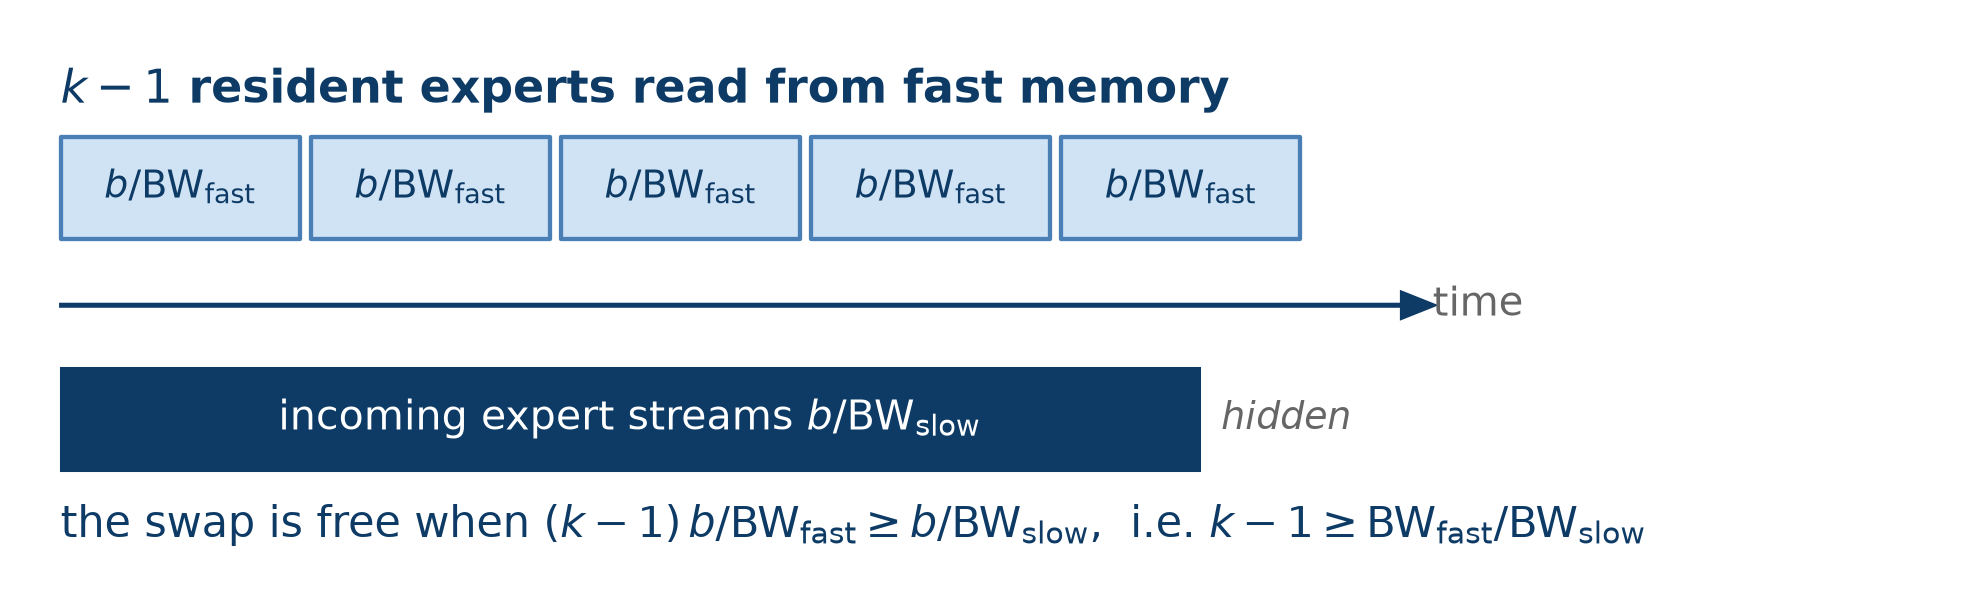
\includegraphics[width=0.88\linewidth]{figures/bandwidth_timeline_nocaption.png}
  \caption{One decode step of one MoE layer under rolling residency. The expert FFN is
  memory-bound at decode, so reading the $k-1$ resident experts occupies
  $(k-1)\,b/\mathrm{BW}_{\mathrm{fast}}$ of wall-clock time while the incoming expert streams
  its $b$ bytes underneath at $b/\mathrm{BW}_{\mathrm{slow}}$. The stream is hidden whenever
  the resident reads take at least as long. The expert size $b$ cancels from the condition,
  so only the routing width $k$ decides it.}
  \label{fig:bandwidth}
\end{figure}

\paragraph{The bandwidth condition.} Figure~\ref{fig:bandwidth} shows the timeline of one
decode step. Serving the $k-1$ already-resident experts reads $(k-1)\,b$ bytes from fast
memory while the incoming expert streams its $b$ bytes from slower storage, and the swap is
free when $b/\mathrm{BW}_{\mathrm{slow}}\le(k-1)\,b/\mathrm{BW}_{\mathrm{fast}}$, that is,
once $k-1$ reaches the bandwidth ratio of the tier pair it streams across. The expert size
$b$ cancels, so the condition depends only on the routing width $k$, the knob that
granularity scaling laws quantify
\citep{krajewski2024granularity,clark2022unified,ludziejewski2025joint}. Our fine-grained
models route 18 of 192 experts, which puts $k-1=17$ at the low end of the 15-to-100 ratios
common between memory tiers, and each split expert is smaller, so a swap also moves fewer
bytes. Section~\ref{sec:serving} profiles the tiers of two real devices and tests the
condition end to end, including a variant that computes the router earlier in the network
than its experts to lengthen the masking window.

\section{Pretraining under the constraint}\label{sec:pretraining}

\paragraph{Setup.} We build on FLAME-MoE \citep{kang2025flame}, an open MoE pretraining suite
whose default layer routes 6 of 64 experts alongside one always-active shared expert, and
train every model at two granularities, the FLAME default and the fine-grained split (18 of
192). At $10^{16}$ and $10^{17}$ FLOPs we sweep isoFLOP curves over 0.77M to 15.1M active
non-embedding parameters with a 16k vocabulary. At $10^{18}$ we sweep three sizes around an
exact replication of FLAME-MoE-38M-100M (4.45B tokens, 50k vocabulary), giving the
compute-optimal midpoint three seeds per model and the flanks one. At $10^{19}$ we train the
budget's compute-optimal shape. Every shape gets a dense floor matched to the MoE's active
parameters and FLOPs, hyperparameters are locked across paradigms, and quality is test-set
bits per byte (BPB), which is tokenizer-invariant. Seed noise is about 0.003 BPB. Recovery,
used throughout, is $(\text{dense}-\text{temporal})/(\text{dense}-\text{MoE})$, the share of
the MoE-over-dense gain the constrained model keeps.

\begin{figure}[t]
  \centering
  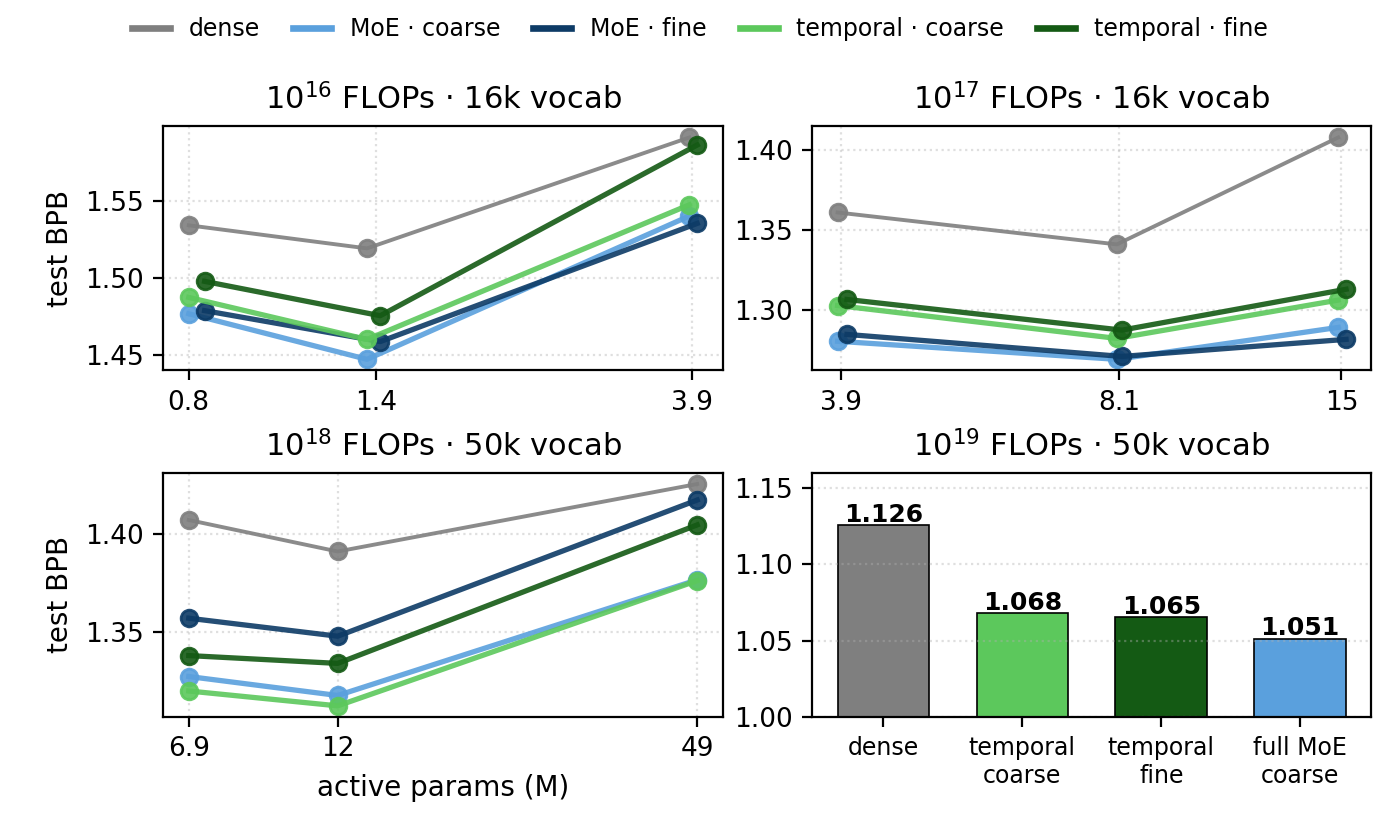
\includegraphics[width=0.82\linewidth]{figures/isoflop_panels_2x2_nocaption.png}
  \caption{Quality at fixed compute, one panel per budget (test-set BPB, lower is better).
  Gray is dense, blue full MoE, green temporal, and darker shades are the fine granularity
  (18 of 192). Vocabularies differ between budgets, so BPB is comparable within a panel, not
  across. Temporal MoE lands inside the dense-to-MoE band at every size and budget. The
  $10^{18}$ midpoints plot three-seed means (Appendix~\ref{app:seeds}).}
  \label{fig:isoflop}
\end{figure}

\paragraph{IsoFLOP bands.} At every model size in the three budgets with full sweeps
(Figure~\ref{fig:isoflop}), temporal MoE lands inside the dense-to-MoE band and keeps 72 to
82\% of the MoE-over-dense gain at the compute-optimal sizes, 82\% at the coarse granularity
in both smaller budgets and 72 to 77\% at the fine one. The isoFLOP parabola and its minimum
match the dense and MoE baselines at every budget, so the constraint leaves the scaling
geometry essentially unchanged.

\paragraph{Larger budgets.} At $10^{18}$ FLOPs the coarse temporal model reaches parity with
the strongest full MoE (seed means 1.312 against 1.317 BPB) and the fine temporal model lands
below its equally fine full-MoE counterpart (1.334 against 1.348), with seed spread under
0.004 BPB in every model (Appendix~\ref{app:seeds}). Measured against the strongest full MoE,
fine temporal recovery is 78\%, consistent with the smaller budgets. The within-granularity
win is a single-budget observation and we do not build on it. Fine-graining itself hurts the
full MoE at this scale, where at 48.5M active parameters the fine full MoE lands within 0.008
BPB of the dense floor, while temporal routing tolerates it, so the only fine-grained model
we take to $10^{19}$ is the temporal one. At $10^{19}$, our largest budget, the temporal
models keep 78 to 81\% of the gain and the granularity preference flips, with the fine model
(1.065 BPB) edging the coarse one (1.068).

\paragraph{Downstream accuracy.} Zero-shot accuracy at $10^{19}$ (Table~\ref{tab:lmeval})
tracks the pretraining picture. The full MoE lifts the dense six-task average from 0.392 to
0.424 (0.059 to 0.091 above chance), and the temporal models keep 86\% (coarse) and 76\%
(fine) of that above-chance gain. The dense-to-MoE average gap spans several standard errors
while the MoE-to-temporal gaps sit within one, so the lift over dense is statistically clean
and the residual temporal deficit is not resolved at this scale.

\begin{table}[t]
  \centering\small
  \caption{Zero-shot accuracy at $10^{19}$ FLOPs (lm-evaluation-harness, acc\_norm except
  WinoGrande, which reports acc). Avg$-$chance subtracts each task's chance floor (0.5 for
  WinoGrande and PIQA, 0.25 elsewhere) before averaging. Bold marks the best per column.
  Per-task standard errors are 0.005 to 0.020, so single-task bold margins of a point or two
  sit within noise and the aggregate columns carry the comparison.}
  \label{tab:lmeval}
  \vspace{4pt}
  \begin{tabular}{@{}lrrrrrrrr@{}}
    \toprule
    model & OBQA & WinoG & PIQA & ARC-e & ARC-c & HSwag & Avg & Avg$-$chance \\
    \midrule
    dense                 & .276 & .501 & .621 & .437 & .222 & .296 & .392 & .059 \\
    full MoE, 6 of 64     & \textbf{.296} & .507 & \textbf{.659} & \textbf{.495} & .247 & \textbf{.341} & \textbf{.424} & \textbf{.091} \\
    temporal, 6 of 64     & .292 & \textbf{.512} & \textbf{.659} & .473 & .246 & .336 & .420 & .086 \\
    temporal, 18 of 192   & .288 & .487 & .652 & .481 & \textbf{.254} & .336 & .416 & .083 \\
    \bottomrule
  \end{tabular}
\end{table}

\paragraph{The constraint is a dial.} Decoupling the resident budget $R$ from the active $k$
interpolates between the deployed setting ($R=k$) and the full-MoE recipe ($R=E$) at
identical FLOPs. Held-out BPB falls monotonically as the cache grows (Figure~\ref{fig:dose}),
the full 10.7-fold range of resident memory costs 0.023 BPB end to end, and most of that
arrives in the final doubling toward $R=E$. Because $R$ counts the experts held in fast
memory, the curve doubles as the serving memory-quality frontier, and its flatness at the
tight end is what makes the deployed $R=k$ an efficient operating point. Expert diversity
survives every dose, with 182 to 186 effective experts of 192. Auxiliary losses that reward
cache-friendliness directly, tried in place of the hard constraint, all lost quality and
reduced the effective experts (Appendix~\ref{app:negatives}).

\begin{figure}[t]
  \centering
  
\includegraphics[width=0.5\linewidth]{figures/residency_dose_curve_nocaption.png}
  \caption{Held-out BPB against resident budget $R$ at identical FLOPs (192 experts, $k=18$,
  $10^{16}$ FLOPs, every dose trained from scratch). Lower is better. $R$ is the
  resident-expert memory, so this curve is the serving memory-quality frontier.}
  \label{fig:dose}
\end{figure}

\section{What the router learns instead}\label{sec:mechanism}

Section~\ref{sec:pretraining} priced the constraint. This section investigates how routing
reorganizes to pay so little. Every measurement runs on a fixed evaluation batch per model,
probes are fit per expert and scored on held-out documents (chance 0.5), and protocols, null
controls, and full tables are in Appendix~\ref{app:probes}.

\paragraph{The router prefers the locality it is constrained to.} Figure~\ref{fig:locality}
(left) rasters the experts active at each token over a long sequence, at the deepest MoE
layer of an 8.1M-active model. The full MoE scatters. The temporal resident set forms long
streaks, and the temporal router's unconstrained preference, read with the residency mask
removed, is streaked as well, so the trained router prefers stable experts rather than merely
tolerating the ones it is given. The rest of this section quantifies that reorganization.

\paragraph{The resident set anticipates demand, more so with depth.} Hit rate is the share of
a token's unconstrained top-$k$ already resident before any swap, floored at $k/E=0.094$ by a
random resident set. The temporal router reaches 0.32 against 0.17 for the matched full MoE
(Figure~\ref{fig:locality}, right). Hit rate also rises with depth in both regimes, roughly
doubling from the shallowest MoE layer to the deepest. That is an inductive bias with a
serving consequence, since a memory budget rationed across layers buys the most where caching
is hardest, in the shallow layers.

\begin{figure}[t]
  \centering
  \begin{minipage}[t]{0.47\linewidth}
    \centering
    
\includegraphics[width=\linewidth]{figures/expert_selection_per_token_8M_model_nocaption.png}
  \end{minipage}\hfill
  \begin{minipage}[t]{0.47\linewidth}
    \centering
    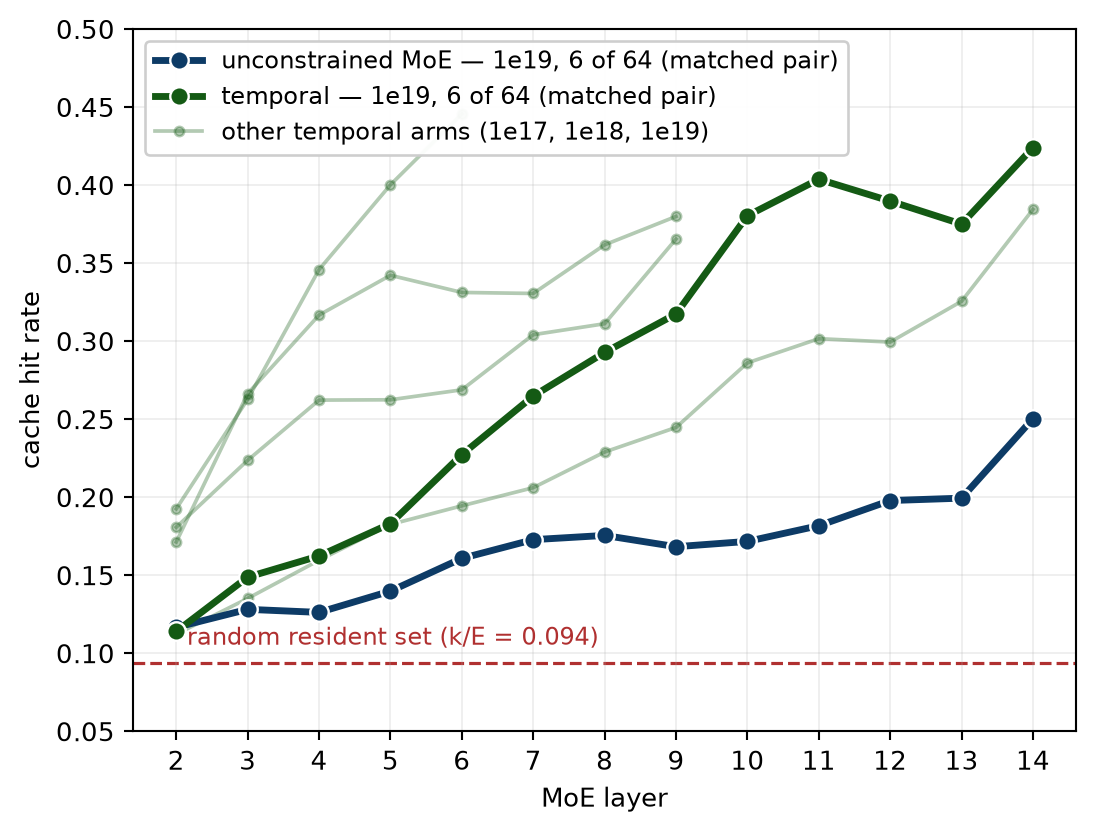
\includegraphics[width=\linewidth]{figures/hitrate_by_layer_nocaption.png}
  \end{minipage}
  \caption{\textbf{Left,} experts active per token (8.1M-active model, deepest MoE layer).
  The vanilla full MoE (top) scatters, the temporal resident set (middle) forms long streaks,
  and the temporal router's unconstrained preference with the mask removed (bottom) is also
  streaked, so the preference for stable experts is trained into the router rather than
  forced at each step. \textbf{Right,} cache hit rate by MoE layer, the share of a token's
  unconstrained top-$k$ already resident before any swap, against the $k/E=0.094$ random
  floor (higher is better). Dark lines are the matched 6-of-64 pair at $10^{19}$, light lines
  the other temporal models. Hit rate roughly doubles with depth in both regimes.}
  \label{fig:locality}
\end{figure}

\paragraph{Token identity fades from the routing signal.} For each expert, two probes predict
whether it fires, one from the current token's embedding alone and one from the mean of the
surrounding tokens with the current token excluded. Across 34 trained models the token axis
separates the regimes completely, with an empty band 0.184 wide holding no model of either
kind (Figure~\ref{fig:armsep}), while the context axis does not separate them at all. Median
token AUC falls from 0.884 in the unconstrained models to 0.585 in the temporal ones while
context AUC moves only from 0.640 to 0.697, so the constraint mostly removes the token signal
rather than adding a context signal. The change also has a depth structure, with
unconstrained routing growing more contextual layer by layer while temporal routing is
contextual from the shallowest MoE layer on (per-layer curves in Appendix~\ref{app:probes}).

\begin{figure}[t]
  \centering
  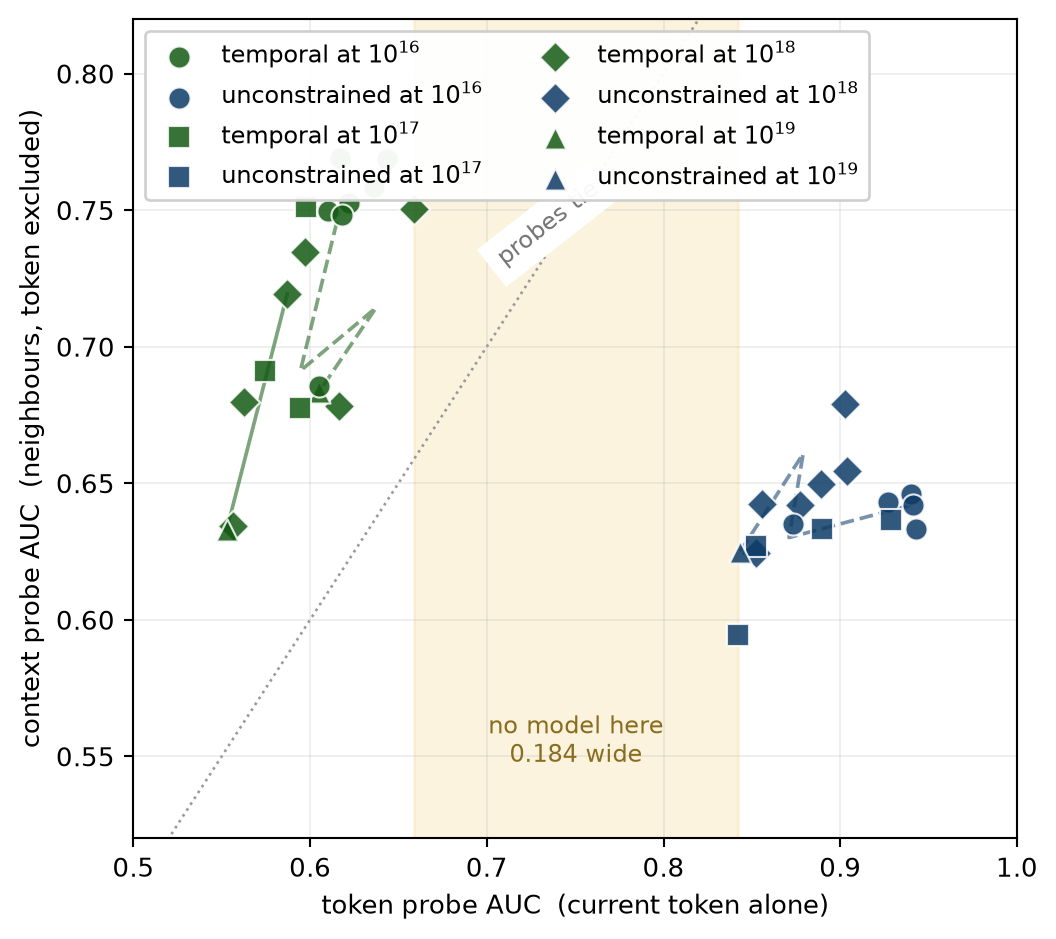
\includegraphics[width=0.58\linewidth]{figures/arm_separation_nocaption.png}
  \caption{One point per trained model, 34 models across four budgets and both granularities.
  Horizontal, how well the current token alone predicts expert firing (median per-expert AUC,
  held out on unseen documents, chance 0.5). Vertical, the same for the surrounding context
  with the token excluded. The shaded band on the token axis is empty, 0.184 wide, and
  separates every temporal model from every unconstrained one, while the context axis separates
  nothing.}
  \label{fig:armsep}
\end{figure}

\paragraph{Experts spread across the stream.} Participation ratio, the inverse Simpson index
of an expert's token distribution on a 0-to-1 scale, measures how much of the stream an
expert serves. The median expert of the fine-grained full MoE serves an effective 30\% of
tokens, its temporal counterpart 66\%, and the coarse pair moves the same way (all configurations in
Appendix~\ref{app:probes}). A training control that runs the full temporal schedule while
constraining zero layers lands with the full-MoE models, so the shift tracks the constraint
rather than the training configuration. Expert weights themselves barely move, with centroid
distance and pairwise cosine indistinguishable between regimes, so the constraint changes how
experts are used far more than what they compute.

\paragraph{Smoother weights, cheaper bits.} The spread usage shows up in the weights. Excess
kurtosis of the routed-expert weight matrices, 0 for a Gaussian, is lower for the temporal
model in every matched pair, with medians of 0.14 against 0.42 for the coarse pair and 0.24
against 0.62 for the fine pair at $10^{18}$, and the gap widens in the tail, where the 99th
percentile falls from 2.79 to 0.77. Fewer outliers make quantization cheaper. Under per-group
round-to-nearest on routed experts only (Figure~\ref{fig:fakequant}), 8-bit is lossless in
both regimes, and at 4 and 3 bits the temporal model degrades less than its matched full MoE
in all three pairs, at both granularities and both scales measured. The two memory levers,
residency and precision, compose rather than trade off, which matters because they are the
obvious pair to reach for together.

\begin{figure}[t]
  \centering
  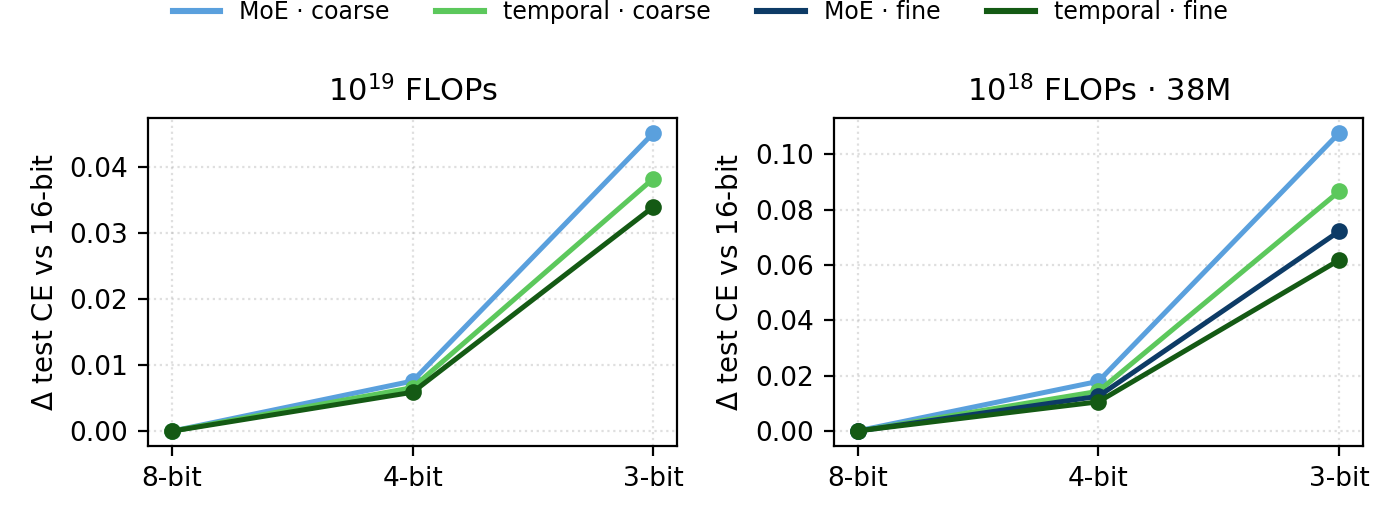
\includegraphics[width=\linewidth]{figures/fakequant_degradation_nocaption.png}
  \caption{Test-CE cost of quantizing routed-expert weights (per-group round-to-nearest,
  group 128), lower is better. Panels have independent scales. The temporal model sits below
  its matched full MoE at every bit width.}
  \label{fig:fakequant}
\end{figure}

\section{Serving}\label{sec:serving}

\paragraph{Setup and devices.} We implement rolling residency in a llama.cpp CUDA fork and
benchmark batch-1 prefill and decode on random-weight Qwen3-MoE-shaped models of matched
total size ($\sim$11.3B, Q4\_K\_M) at both granularities, since weights are irrelevant to a
latency and memory measurement. On an RTX A6000, $R=k$ expert slots live in VRAM, the full
pool lives in CPU RAM, and at most one expert per layer per token streams across PCIe
(840\,KiB per fine swap, 2.5\,MiB per coarse). Prefill runs expert-major, so each needed
expert streams once and serves all of its tokens in one batched pass. On a Pixel 10a phone
the same discipline runs CPU-only, with $R$ slots in RAM and experts streamed from UFS flash
(measured 1.9\,GB/s cold sequential) by direct reads. Both stacks are gated on exactness,
with decode bit-identical to the stock all-resident engine, and the phone's fetched bytes
verified against device-level disk counters.

\begin{table}[t]
  \centering\small
  \caption{Decode throughput at 1024-token context (tok/s, RTX A6000, batch 1). Deploy holds
  only the $R=k$ active experts in VRAM, 1502 against 7672\,MiB, a 5.1$\times$ total and
  10.6$\times$ expert-tier reduction, and streams the rest from a CPU pool. The
  vanilla-offload row is the same memory budget without the trained constraint, free top-$k$
  routing with every miss fetched at the $\sim$20\% consecutive overlap of released MoEs
  (Appendix~\ref{app:serving}).}
  \label{tab:serving}
  \vspace{4pt}
  \begin{tabular}{@{}lrrrr@{}}
    \toprule
    setup & fine 18-of-192 & vs ceiling & coarse 6-of-64 & vs ceiling \\
    \midrule
    all experts in VRAM (ceiling) & 200 & 1.00$\times$ & 252 & 1.00$\times$ \\
    our kernel, no swaps          & 176 & 0.88$\times$ & 217 & 0.86$\times$ \\
    deploy: active-only in VRAM   & \textbf{165} & \textbf{0.83$\times$} & 128 & 0.51$\times$ \\
    router-early variant          & 173 & 0.87$\times$ & 143 & 0.57$\times$ \\
    vanilla offload: active-only, free routing & 43 & 0.22$\times$ & 42 & 0.17$\times$ \\
    \bottomrule
  \end{tabular}
\end{table}

\paragraph{Decode on the workstation GPU.} Table~\ref{tab:serving} closes the loop the
bandwidth condition opened. The deploy row serves the fine-grained model at 0.83$\times$ the
all-resident decode speed in 5.1$\times$ less VRAM, the measured counterpart of the
5.7$\times$ whole-model arithmetic from the resident-set accounting, with the gap being KV
cache and workspace buffers that sit in VRAM regardless of residency. The other rows isolate
the two costs. Kernel overhead is granularity-independent at 0.86 to 0.88$\times$, while the
streaming cost is set by granularity, nearly hidden for fine experts and dominant for coarse
ones (0.51$\times$), which is the bandwidth condition of Section~\ref{sec:method} made
visible. The vanilla-offload row shows the same memory budget without the trained
constraint, where free routing misses most of its experts every token and runs 3 to
4$\times$ slower than deploy. The router-early variant, which computes each layer's routing
before attention so the swap overlaps more compute, recovers most of the fine model's
remaining gap in the engine. Training that architecture in from scratch failed, however,
costing +0.04 BPB on the temporal model and +0.15 on the full MoE at $10^{18}$ FLOPs
(Appendix~\ref{app:negatives}), so we report the engine row as an upper bound on what
overlap could buy, not as a viable design.

\paragraph{Prefill and long context.} Figure~\ref{fig:servingctx} extends the measurement
across context lengths. Prefilling 16k tokens takes 1.6$\times$ the all-resident time,
decode holds near 0.80$\times$ throughout, and peak VRAM stays under 3.6\,GiB against 8.0 to
9.3\,GiB all-resident, a gap the growing KV cache compresses from 3.7$\times$ at 1k tokens
to 2.6$\times$ at 16k. At larger batch each sequence carries its own resident set, so the
advantage narrows there as well. Micro-batch choice, the prefill time decomposition, and the
vanilla-offload floor curve are in Appendix~\ref{app:serving}.

\begin{figure}[t]
  \centering
  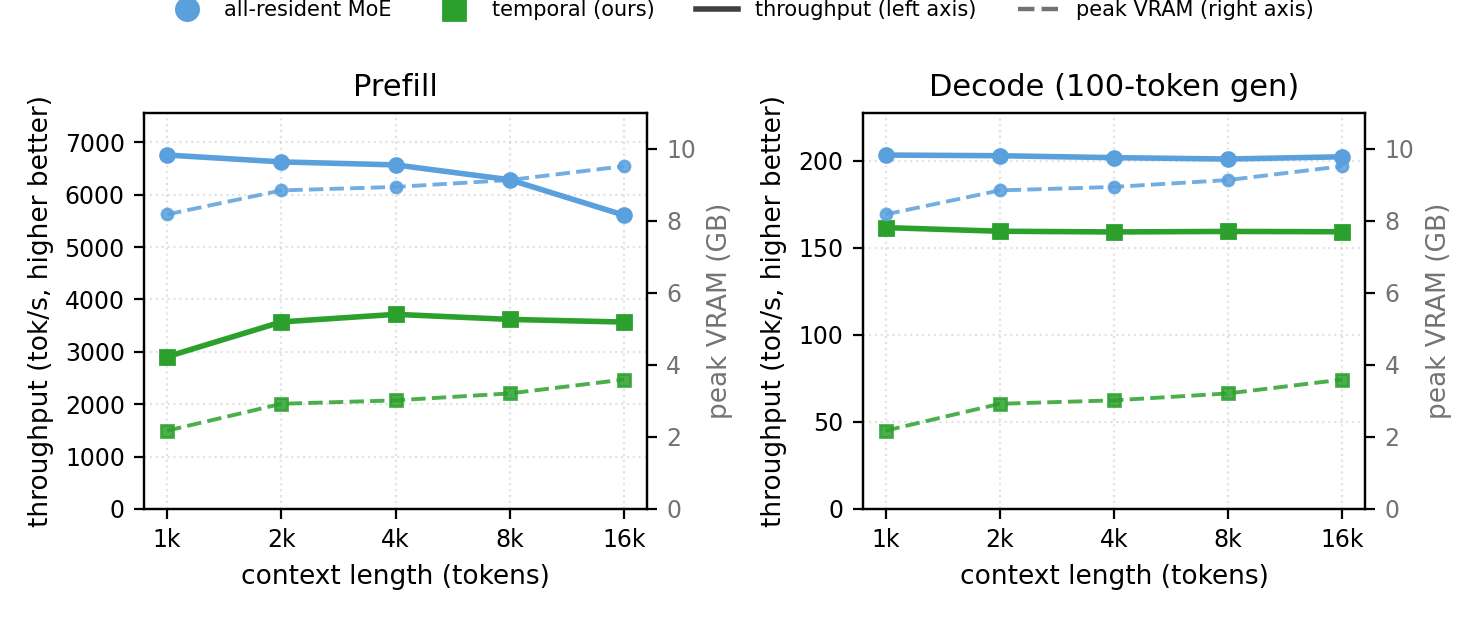
\includegraphics[width=\linewidth]{figures/serving_context_sweep_nocaption.png}
  \caption{Serving against context length, fine-grained model on the RTX A6000. Solid lines
  are throughput (left axis), dashed lines peak VRAM (right axis). Decode runs after the
  full prefill, slightly below Table~\ref{tab:serving}'s decode-only setting.}
  \label{fig:servingctx}
\end{figure}

\paragraph{A phone the model does not fit in.} The Pixel 10a has 7.75\,GB of RAM and about
3.6\,GB available, against a 5.5\,GiB model, and the all-resident baseline cannot run at
all, with the one attempt panicking the kernel. Temporal residency is what makes the model
servable on this class of device. Streaming from flash, decode reaches 10.5 tok/s at $R=36$
(a 5.3$\times$ expert-memory cut) and 11.8 at $R=64$ (3$\times$), which is 60 to 71\% of an
all-resident ceiling that has to be inferred from byte accounting because it cannot be
measured. Two caveats bound the claim. The ceiling is inferred, not run, and the
random-weight router swaps 2.09 experts per layer, roughly twice the $\sim$1-swap design
point of a trained temporal router, so these rates understate what a trained model would
reach, with the tightest $R=k$ point (5.65 tok/s, about a third of the ceiling) taking most
of that penalty.

\paragraph{One design point.} Scale pushes temporal quality toward fine granularity
(Section~\ref{sec:pretraining}), and fine granularity is what streams cheaply, on the A6000
because an 840\,KiB swap hides behind resident compute where a 2.5\,MiB one does not, and on
the phone because smaller experts keep the per-swap flash read inside the fetch-hiding
window. Quality and serving select the same design point, which is the paper's central
alignment.

\section{Released instruct models under residency}\label{sec:instruct}

\paragraph{Setup.} We impose the decode-time protocol of Section~\ref{sec:method} on six
released instruct MoEs, ordered by total size: OLMoE-1B-7B-Instruct (64 experts, $k=8$),
LFM2.5-8B-A1B (32, $k=4$), gpt-oss-20b (32, $k=4$), gemma4-26B-IT (128, $k=8$),
Qwen3.5-35B-A3B (256, $k=8$), and gpt-oss-120b (128, $k=4$). Each model runs three settings.
Free routing is the reference. $R=k$ is the tightest valid cache, since with fewer residents
than $k$ the router cannot fill its own top-$k$. $R=12.5\%$ of the expert pool is the
common-denominator setting: the sparsest models in the panel already have $k/E=4/32=12.5\%$, so
12.5\% is the tightest fraction every model can share, and for those two models the settings
coincide. Every thinking-capable model runs both of its modes, thinking off against on for
gemma4 and Qwen3.5 and low against high effort for the gpt-oss pair, on the same items and settings;
LFM thinks natively with no toggle, and OLMoE has no thinking mode. Surfaces are GSM8K,
IFEval, HumanEval, MMLU, and WritingBench, run under each
model's own model-card sampling recipe
with single-pass generation at per-task budgets, MMLU scored by answer extraction rather
than the stock strict format filter, and HumanEval parsed channel-aware for models that
think in-band. WritingBench ran with thinking off and its deltas are critic points on
a 1-to-10 scale, multiplied by 10 wherever they enter a shared axis with the accuracy
benchmarks. Cells are single runs with binomial standard errors of 2 to 4 points, and the
full protocol and its measurement corrections are in Appendix~\ref{app:instrproto}.

\begin{figure}[t]
  \centering
  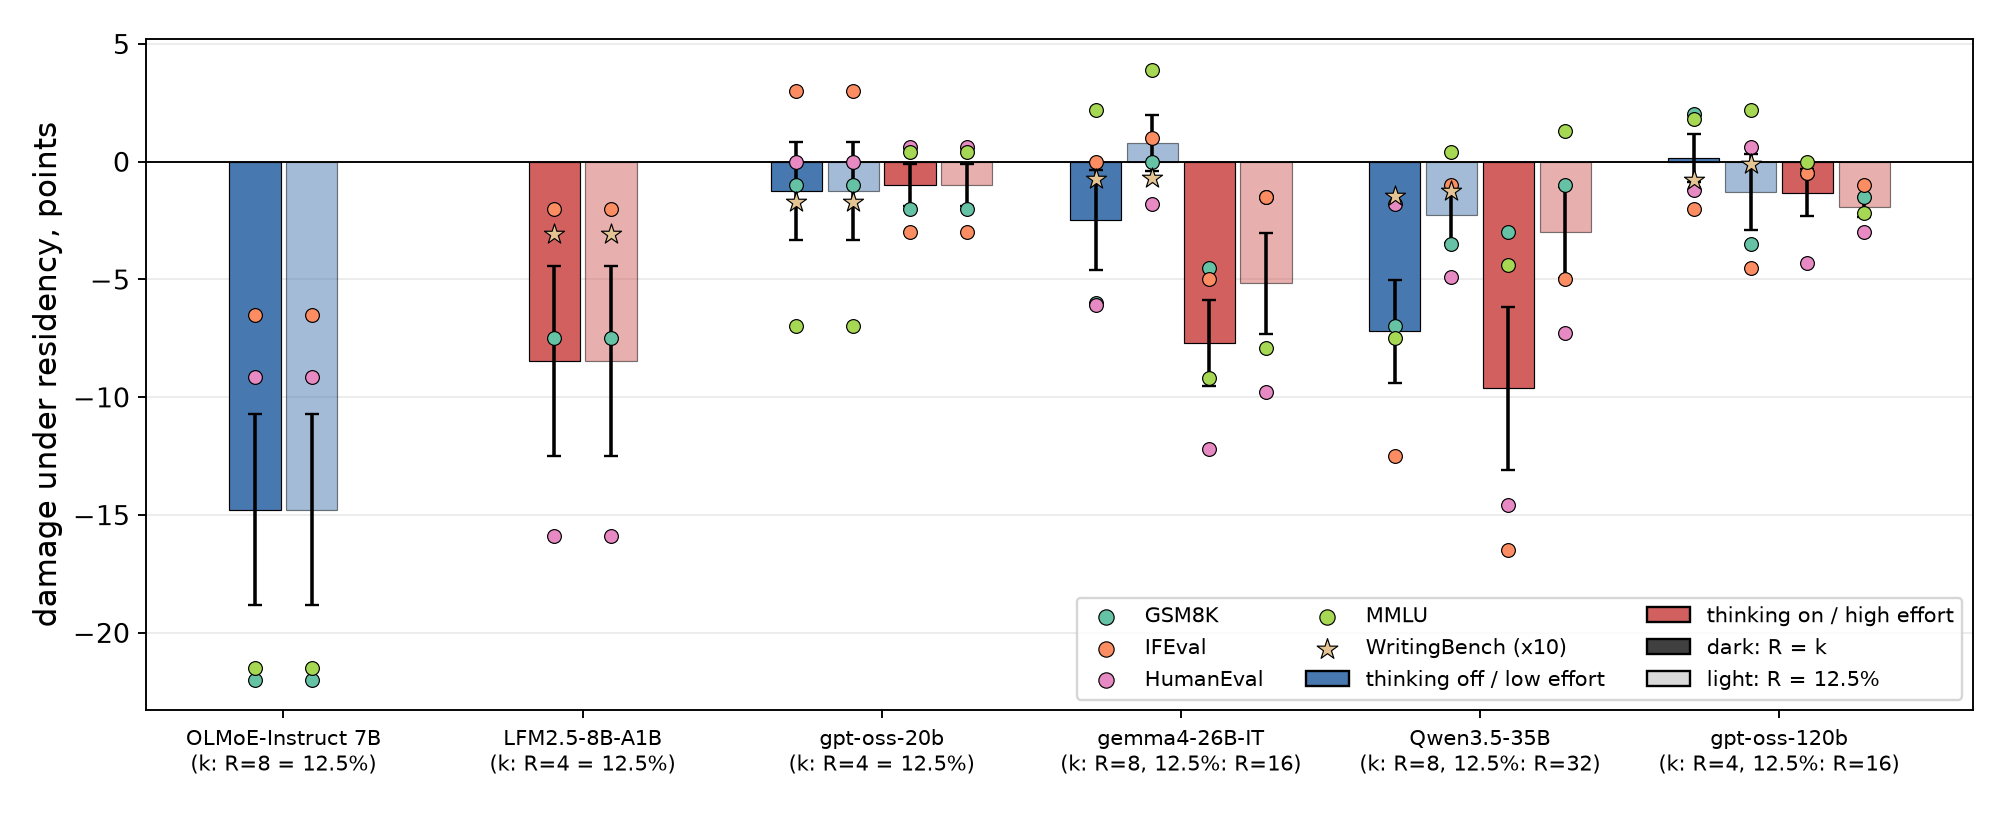
\includegraphics[width=0.97\linewidth]{figures/instruct_model_damage_nocaption.png}\\[4pt]
  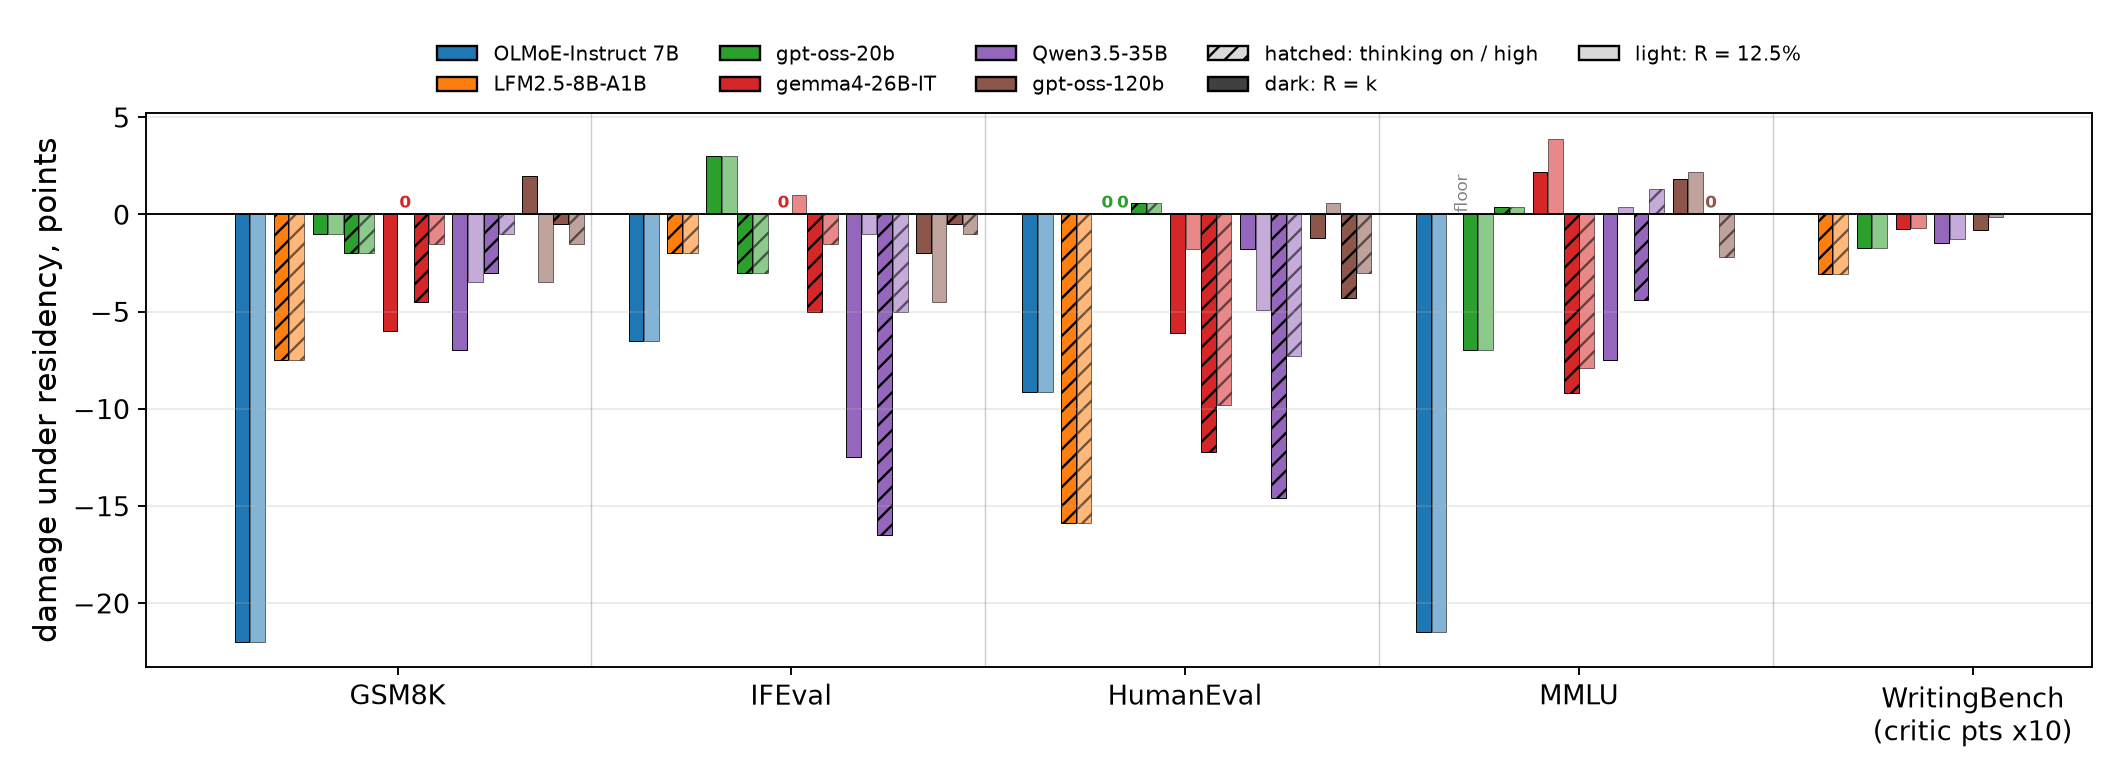
\includegraphics[width=0.97\linewidth]{figures/instruct_bench_damage_nocaption.png}
  \caption{Damage under decode-time residency (constrained minus free, points), models
  ordered by total size, dark bars $R=k$ and light bars $R=12.5\%$ of experts, blue bars
  thinking off or low effort and red bars on or high. \textbf{Top,} per model: bars are the
  mean over the four accuracy benchmarks, whiskers the standard error of that mean from the
  surface spread, dots the per-surface deltas, and stars the WritingBench critic deltas
  $\times$10 (thinking-off runs, shown as points and not in the means). For the three models
  where $k/E=12.5\%$ the two settings coincide. \textbf{Bottom,} the same measurements per benchmark,
  color per model and hatching for the thinking-on and high-effort modes. LFM's MMLU
  sits at its extraction floor and is omitted. Single runs, binomial standard errors 2 to 4
  points.}
  \label{fig:instrdamage}
\end{figure}

\paragraph{Survivable without training, priced by fraction.} Figure~\ref{fig:instrdamage}
(top) gives the summary view. With thinking off or at low effort, mean damage over the four
accuracy benchmarks at $R=k$ is $-14.8$ points for OLMoE, $-1.2$ for gpt-oss-20b, $-2.5$ for
gemma4, $-7.2$ for Qwen3.5, and $+0.2$ for gpt-oss-120b, with LFM's native mode at $-8.5$,
so the strongest models pay a few points for a serving cache no larger than their active
experts, with no training of any kind. Relaxing to 12.5\% of the pool recovers most of what
the tightest setting loses where the two differ, gemma4 to $+0.8$ and Qwen3.5 to $-2.2$. What sets the
price of the tightest setting is the residency fraction rather than the slot count. Qwen3.5's $R=8$ is 3.1\%
of its 256 experts and loses nearly three times gemma4's mean at $R=8=6.25\%$.

\paragraph{Free-form thinking amplifies the constraint, effort control does not.} The red
bars in Figure~\ref{fig:instrdamage} carry the second axis. Turning thinking on roughly
triples gemma4's mean at $R=k$, $-2.5$ to $-7.7$, and deepens Qwen3.5's, $-7.2$ to $-9.6$,
while the gpt-oss models' effort dial barely moves the price, $+0.2$ to $-1.3$ at 120b and
$-1.2$ to $-1.0$ at 20b. The per-benchmark rows show where the amplification lives, in
IFEval and HumanEval, with Qwen3.5's thinking IFEval at $-16.5$ the worst single result of the panel.
Relaxing to 12.5\% shrinks the thinking penalty as it does everything else, though gemma4's
thinking-on setting keeps a residual $-5.2$. The generation-length side of this, constrained
thinking chains running 1.1 to 1.3$\times$ longer with nothing bought back, is analyzed in
Section~\ref{sec:length}, and the serving guidance is direct: at tight residency, serve
thinking off or under effort control.

\paragraph{Damage is capability-weighted, and prose is the robust surface.}
Figure~\ref{fig:instrdamage} (bottom) breaks the same measurements out per benchmark. The losses
concentrate in math, code, and instruction following, while MMLU stays within a few points
for every model but OLMoE, so the constraint mostly taxes generative capability rather than
stored knowledge. The WritingBench group is the flattest on the axis even after its
$\times$10 rescaling, with critic costs of $-0.07$ to $-0.31$ points on the 1-to-10 scale at
$R=k$ against accuracy losses of up to 16 points on the same models. The one fluency symptom
we found is a rise in 3-gram loops in Qwen3.5's constrained generations, from 3.5\% to 5.7\% of
responses at $R=8$, which adaptation later removes.

\paragraph{Damage tracks substitutable capacity.} Self cross-entropy (self-CE), each
model's cross-entropy on its own frozen responses, isolates the constraint from benchmark harnesses
(Figure~\ref{fig:instrselfce}). At the matched 12.5\% fraction the damage is 0.94 nats per
token for OLMoE, 0.31 for LFM2.5, 0.21 for gemma4, and 0.11 for Qwen3.5. The ordering
favors models with more routed experts and an always-resident shared expert, and the model
furthest out of line with pure expert count, OLMoE, is the one whose free router leans
hardest on token identity when probed as in Section~\ref{sec:mechanism}. This is the
released-model face of the pretraining picture, where fine granularity tolerated the
constraint best, and it points the same direction the field is already moving, toward more
and smaller experts.

\begin{figure}[t]
  \centering
  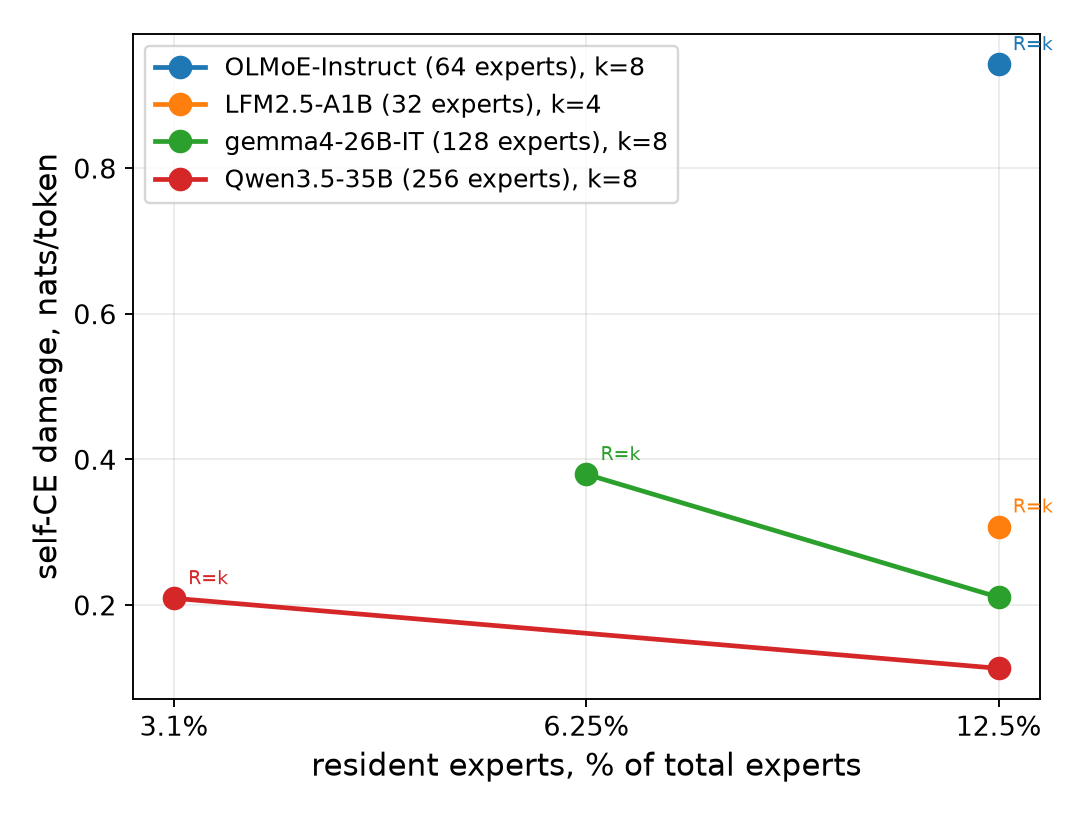
\includegraphics[width=0.52\linewidth]{figures/instruct_selfce_damage_nocaption.png}
  \caption{Self cross-entropy damage on each model's own frozen responses (nats per token,
  lower is better) against resident fraction, $R=k$ marked per model. At the matched 12.5\%
  fraction the spread is nine-fold.}
  \label{fig:instrselfce}
\end{figure}

\paragraph{Tolerance is predictable before any benchmark runs.} A natural guess is that
models whose router probabilities move most under the mask suffer most. The opposite holds,
with router-distribution displacement anti-ordering benchmark damage across the six models
(Spearman $-0.49$). What orders it is functional displacement, the relative output error of
the routed-expert layer when the resident set substitutes for the free choice on identical
inputs, at Spearman $+0.66$ and exactly ordering damage within each residency fraction
(Appendix~\ref{app:instrproto}). Substitutability of expert function, not stability of
routing probabilities, is what tolerance to the constraint measures, which fits
Section~\ref{sec:mechanism}'s finding that the constraint changes how experts are used far
more than what they compute.

\section{Generation length under the constraint}\label{sec:length}

Section~\ref{sec:instruct} showed that free-form thinking amplifies the constraint's cost.
This section asks what happens to the generations themselves, using per-item paired data:
the same 200 items per configuration, generated free and constrained, with exact token counts.
Per-item capture exists for GSM8K and IFEval on every model, while MMLU and the
family-specific HumanEval harnesses saved no per-item lengths, so this analysis covers math
and instruction following and does not reach code, where Section~\ref{sec:instruct} showed
damage also concentrates. Mean ratios answer the question badly, because the length change
is not one phenomenon.

\paragraph{Two components, not one.} Figure~\ref{fig:lendecomp} decomposes each configuration's mean
per-item length change into the part carried by items at the generation cap under either setting
and the part carried by items that never hit it. The configurations separate cleanly. gemma4 with
thinking on is cap-dominated on both tasks, and LFM nearly so on GSM8K. Qwen3.5 with thinking
on splits roughly in half on IFEval, with 213 tokens per item of broad lengthening across
never-capped items on top of its cap traffic. gpt-oss-120b at high effort lengthens entirely
broadly, with a cap component near zero, and gpt-oss-20b at high effort runs the two
components in opposite directions, cap churn adding length while its normal items shorten.
Thinking-off configurations sit within a few tokens of zero everywhere. Across
configurations the cap part
tracks the total only loosely, so neither component reduces to the other, and both are real.

\begin{figure}[t]
  \centering
  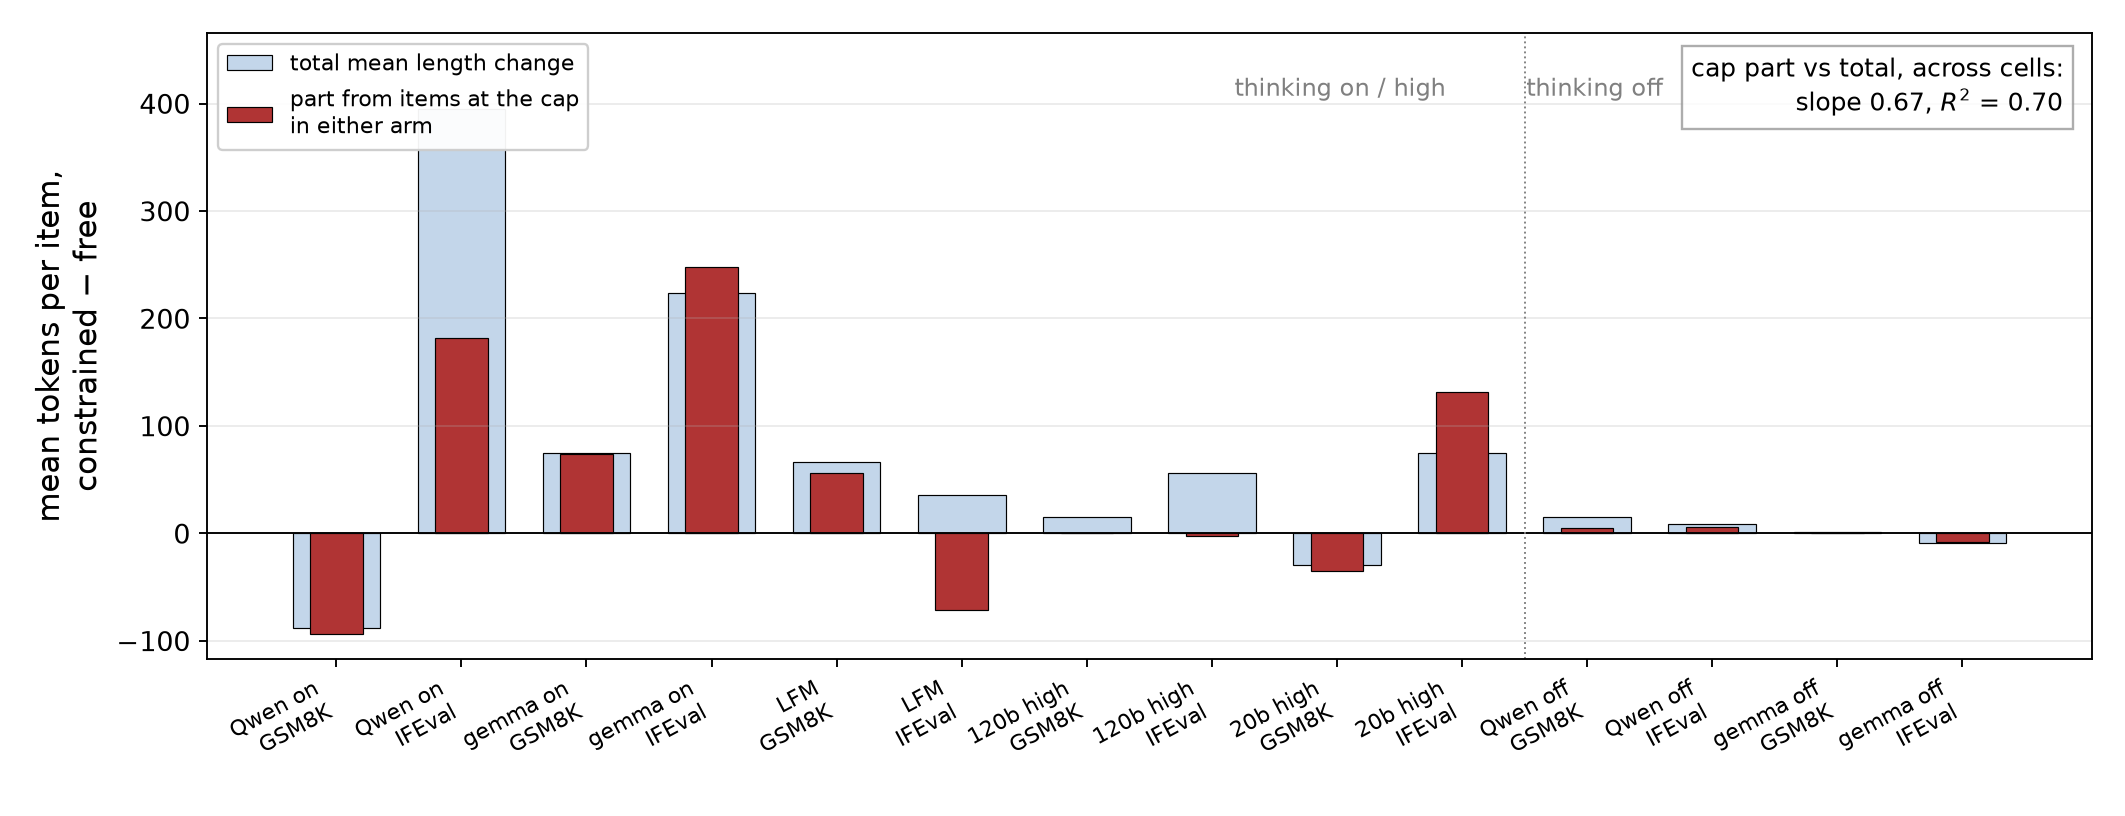
\includegraphics[width=0.95\linewidth]{figures/length_blowup_decomp_nocaption.png}
  \caption{Mean per-item generation-length change under the tight cache (light bars)
  against the part contributed by items at the generation cap under either setting (dark bars),
  paired document ids, 200 items per configuration. The gap between bars is broad lengthening or
  shortening among never-capped items. Across configurations the cap part tracks the total at
  $R^2=0.69$, falling to 0.45 without the two largest, so cap traffic is one
  component of the change, not all of it.}
  \label{fig:lendecomp}
\end{figure}

\paragraph{Where the thinking damage comes from.} Blown-up generations, at the cap or
more than twice their paired counterpart, are wrong more often than normal-length ones in
every thinking configuration under both settings, 20 of 20 comparisons (Appendix~\ref{app:length}). Across
the ten thinking configurations the constraint flips 174 items to wrong against 85 it rescues, so
the reshuffling of who fails is asymmetric in outcome, and Figure~\ref{fig:lenflips} shows
its length signature, with wrong-flips on the blow-up-heavy configurations growing by up to 5{,}300
tokens, rescues being free-routing blow-ups the constrained run avoided, and non-thinking flips
staying length-silent. The mechanism splits by task. On IFEval, where blow-ups concentrate
and the constraint leaves their number per setting nearly unchanged (29 against 34 for Qwen3.5, 14
against 14 for gemma4, 42 against 44 for gpt-oss-20b), 43\% of the flips to wrong are
blow-ups, and the thinking penalty is mostly discrete derailments into the budget wall. On
GSM8K the blow-up share of wrong flips is only 0 to 19\%, so that damage is normal-length
quality loss rather than the wall. Both readings fit the decomposition, since the one configuration
that lengthens broadly with no cap traffic, gpt-oss-120b at high effort, takes no visible
damage, an observation from a single configuration that we do not build on.

\begin{figure}[t]
  \centering
  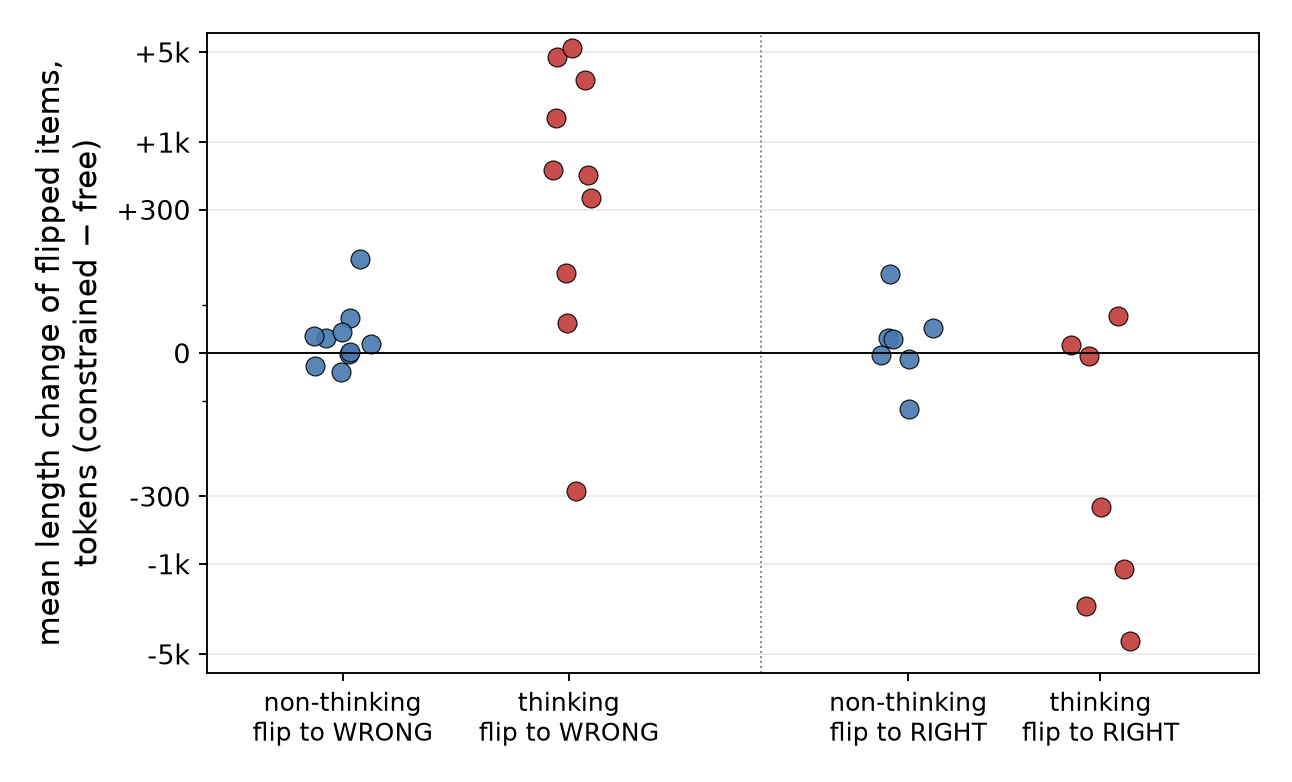
\includegraphics[width=0.62\linewidth]{figures/length_flips_nocaption.png}
  \caption{Mean length change of items whose correctness flipped under the tight cache,
  one point per (model, task) configuration with at least five flips, red for thinking and
  high-effort modes, blue for non-thinking. Thinking flips to wrong mostly grew, thinking
  flips to right are avoided free-routing blow-ups, and non-thinking flips barely move.}
  \label{fig:lenflips}
\end{figure}

\paragraph{Length predicts nothing across tasks.} Across models and benchmarks on exact
token counts, damage at the tightest setting has no significant relationship with how long a
task's responses run under free routing (Spearman $-0.18$, $p=0.63$,
Appendix~\ref{app:length}). An earlier version of this analysis found a significant
correlation and it did not survive the corrected measurement protocol, so we claim the null
and nothing more. Short-answer tasks are not safe and long-form generation is not doomed,
and errors show no sign of compounding over decode length.

The serving guidance of Section~\ref{sec:instruct} follows directly, since the damaged
configurations are the ones whose thinking runs into the budget wall: at tight residency, serve
thinking off or under effort control, and treat generations approaching the cap as likely
failures whichever routing regime produced them. Per-item percentile detail and the
length-damage scatter are in Appendix~\ref{app:length}.


\section{Adapting released models}\label{sec:adaptation}

One GPU-day of constraint-aware finetuning removes most of what
Section~\ref{sec:instruct} measured. The model answers a benchmark-free prompt pool with
thinking off, 9,173 prompts 8-gram-screened against every test set with no truncated rows,
and then trains on its own responses with plain cross-entropy while the constraint is
active on response tokens and prefill stays free, through expert-tensor LoRA r16 on the
expert weight tensors plus attention LoRA r32, with a KL anchor to the base model's
free-routing distribution, for 3.4M response tokens. The constraint during training is the
active ingredient, since the same data with the constraint off gives nothing on this
adapter surface. Figure~\ref{fig:adapt} shows the result. On gemma4 the $R=8$ penalty is essentially erased, GSM8K recovering from $-6.0$ to $0.0$ and HumanEval from $-6.1$ to
$-1.2$ while free-routing quality holds. On Qwen3.5 the same recipe with per-model settings removes
half to two thirds of every damaged measurement, with constrained IFEval at $-6.0$ the one metric
no configuration fixed. WritingBench moves by at most 0.17 critic points in any adapted
measurement, so the repairs cost no fluency. Released MoE checkpoints tolerate the constraint as
they are, and one GPU-day of finetuning removes most of what remains, which turns temporal
routing from a pretraining regime into a serving recipe for existing models.

\begin{figure}[t]
  \centering
  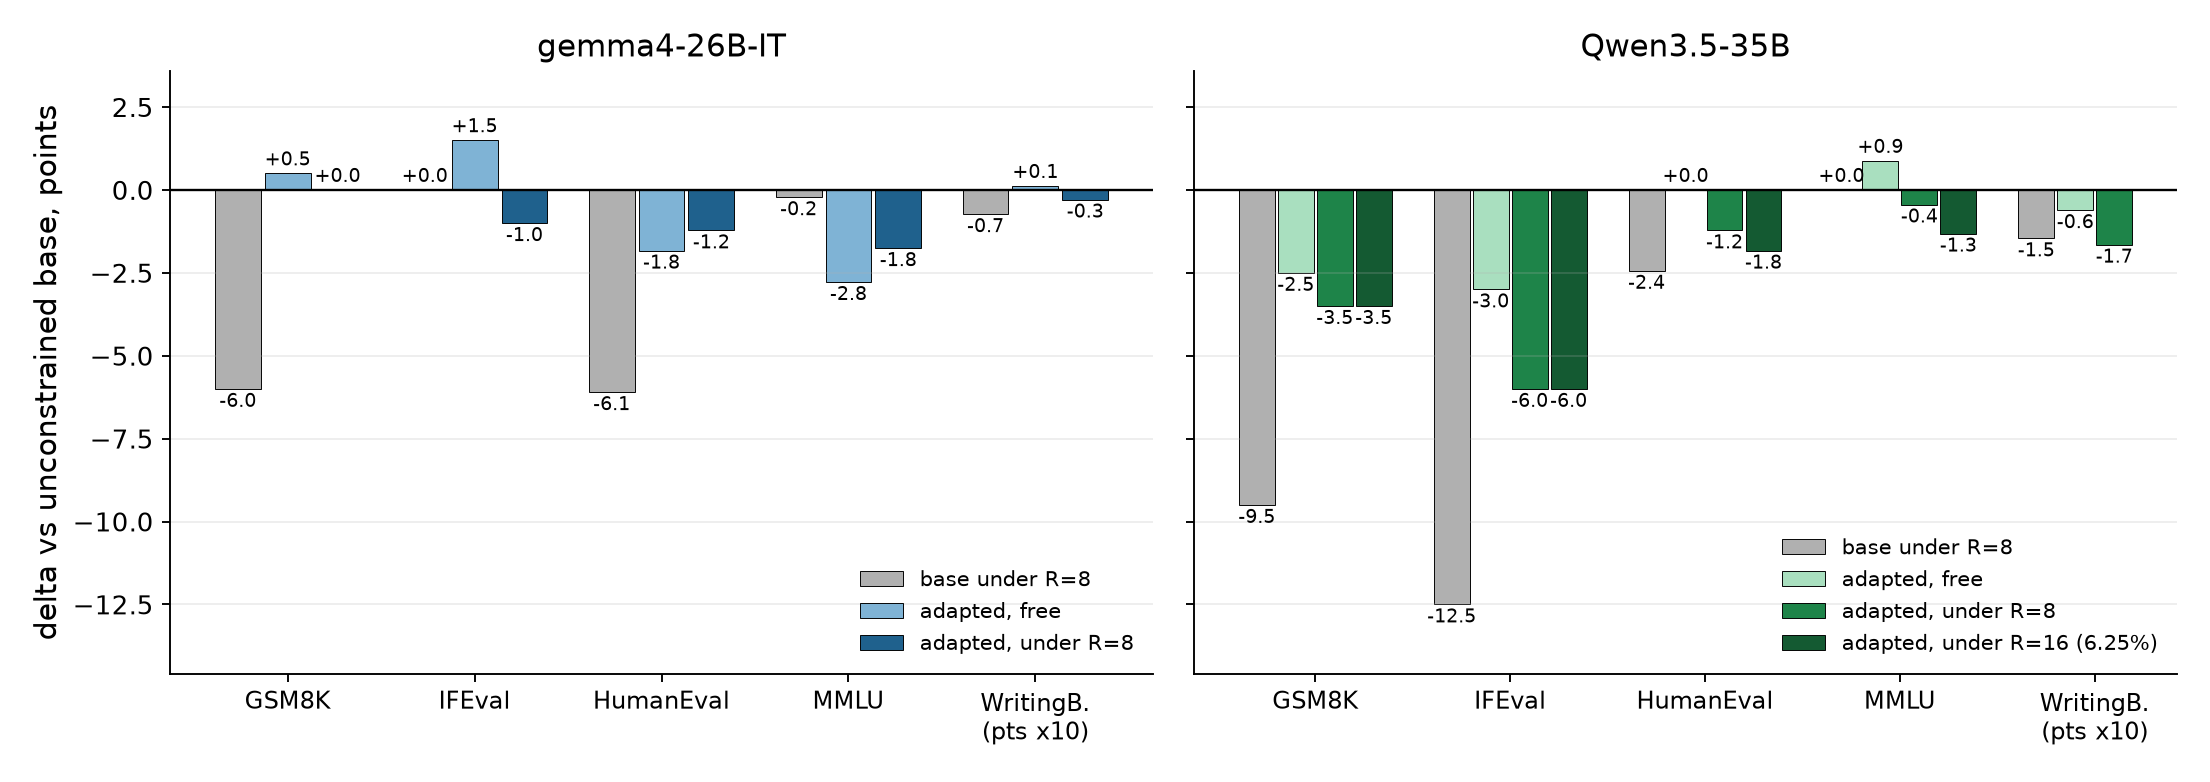
\includegraphics[width=\linewidth]{figures/adapt_combined_nocaption.png}
  \caption{Constraint-aware adaptation against the $R=k$ constraint, per-dataset deltas
  against each model's unconstrained base, WritingBench critic deltas $\times$10. Left,
  gemma4 on the full 200-item evaluation with multi-run MMLU means. Right,
  Qwen3.5 on 200-item screening subsets with same-batch references (single runs, noise $\pm$2
  points), including the fraction-matched $R=16$ setting (6.25\% resident, gemma4's $R=k$
  fraction).}
  \label{fig:adapt}
\end{figure}


\section{Related work}\label{sec:related}

Serving systems keep a pool of $R>k$ experts in fast memory and manage the misses. Eliseev
and Mazur cache experts with LRU and speculative prefetch \citep{eliseev2023}, MoE-Infinity
prefetches from activation traces \citep{xue2024moeinfinity}, ProMoE trains a predictor to
fetch ahead of the router \citep{song2024promoe}, and a survey covers the rest of a crowded
field \citep{liu2024moesurvey}. Skliar et al.\ instead bias a frozen router toward whatever
is cached \citep{skliar2024}. Across this line, locality is a tendency and the pool still
provisions for misses, so the memory footprint remains a knob priced in latency or quality
at serving time. Rolling residency makes the footprint and the swap budget constraints the
model trains under, which is what lets the bandwidth condition of Section~\ref{sec:method}
hold by construction rather than in expectation. Pre-gated MoE overlaps the fetch by
computing each layer's gate one layer early at serving time \citep{hwang2023pregated}. We
find the trained-in version of early routing costly, degrading quality at depth when
trained from scratch (Section~\ref{sec:serving}), so the overlap that line buys on frozen
models does not come free as an architecture.

A newer line shapes the routing itself. Oracle-MoE routes in a compact semantic space so
consecutive tokens pick similar experts \citep{zhou2025oracle}, Sticky Routing and BlockFFN
add losses that penalize switches or shrink the union of experts per chunk
\citep{kayyam2026sticky,song2025blockffn}, CoSMoEs' block-wise selection buys fewer swaps
at a measured quality cost \citep{huber2025cosmoes}, router-only finetuning raises reuse in
released checkpoints \citep{zhu2026reuse,raje2026melinoe}, and a learned controller can
decide when a checkpoint's expert set switches \citep{shen2026temporally}. Our negative
results (Appendix~\ref{app:negatives}) point the same way CoSMoEs' trade does, with soft
objectives that reward cache-friendliness costing quality or collapsing expert diversity
where the hard constraint does neither, and Section~\ref{sec:adaptation} gives the
adaptation line a measured comparison point on standard benchmarks.

A complementary axis serves capacity whose lookup key is known before any compute runs.
Mixture of Lookup Experts re-parameterizes token-conditioned experts into offloaded tables
\citep{jie2025mole}, per-layer embeddings ship the same mechanism in Gemma's edge models
\citep{gemmateam2026}, and Engram scales it to N-gram-keyed memory \citep{cheng2026engram}.
Lookup capacity is lexical by construction, and Section~\ref{sec:mechanism} shows
token-identity binding is exactly what a free router spends experts on and what residency
removes, so the two axes split the problem rather than compete. Tables can hold the
token-keyed capacity while residency streams the context-dependent experts no table can
express, and the combination is natural and untested.

Constraints on routing structure exist along other axes. Path-constrained MoE ties expert
choices across neighboring layers \citep{gu2026pathmoe}, and Mixture-of-Depths spends its
sparsity on skipping compute across the sequence \citep{raposo2024mod}. Residency is the
time-axis member of this family, aimed at serving memory because that is the cost that
binds at deployment.


\section{Conclusion}\label{sec:conclusion}

Across four decades of compute, two tokenizer families, and two expert granularities,
training under rolling residency keeps 72 to 82\% of the MoE-over-dense quality gain while
holding only the active experts resident, preserves the baselines' scaling geometry, and
carries the recovery to downstream tasks. Quality survives because the router reorganizes
rather than degrades, with token identity fading from the routing signal, expert usage
spreading across the pool, and expert weights coming out smoother and cheaper to quantize.
A real serving engine delivers 0.70 to 0.83$\times$ the all-resident decode speed in
5.1$\times$ less memory across a workstation GPU and a phone, and on the phone it makes an
11B-scale model servable at all, since the all-resident model does not fit. Imposed at
decode time, the same constraint costs modern sparse checkpoints a few points, less the
sparser they are, and one GPU-day of constraint-aware finetuning removes most of what
remains, so temporal routing serves as a deployment recipe for existing models as well as a
pretraining regime. The trend also runs in the technique's favor, since the constraint gets
cheaper exactly as released models grow more experts.

The larger motivation for this work is private, local inference. If temporal routing
continues to hold at scale, a sparse model of Kimi-K2 scale \citep{kimik2} could run in the
memory of its active parameters on quantized consumer hardware, putting
near-state-of-the-art capability within the local reach of individual users.


\bibliography{references}
\bibliographystyle{iclr2027_conference}

\appendix

\section{Seed replication and finer granularity at $10^{18}$ FLOPs}\label{app:seeds}

Table~\ref{tab:seeds} lists the runs behind the $10^{18}$ midpoint of
Figure~\ref{fig:isoflop}, all on the same data split.

\begin{table}[h]
  \centering\small
  \caption{Per-seed test BPB at the $10^{18}$ compute-optimal midpoint (lower is better).
  The dense floor is a single run.}
  \label{tab:seeds}
  \vspace{4pt}
  \begin{tabular}{@{}lrrrr@{}}
    \toprule
    & \multicolumn{3}{c}{seed} & \\
    \cmidrule(lr){2-4}
    model & 1 & 2 & 3 & mean \\
    \midrule
    temporal, 6 of 64   & 1.3128 & 1.3111 & 1.3128 & 1.3122 \\
    full MoE, 6 of 64   & 1.3158 & 1.3197 & 1.3169 & 1.3175 \\
    temporal, 18 of 192 & 1.3354 & 1.3339 & 1.3323 & 1.3339 \\
    full MoE, 18 of 192 & 1.3461 & 1.3489 & 1.3483 & 1.3478 \\
    dense               & 1.3911 &        &        & 1.3911 \\
    \bottomrule
  \end{tabular}
\end{table}

A single-variable extension trains both paradigms at 30 of 320 experts on the same budget
and split. The temporal model reaches 1.3491 against 1.3625 for the full MoE, so the
temporal advantage at this granularity (0.013 BPB) matches the replicated 18-of-192 gap
(0.014) and sits above the observed seed ranges of 0.003 to 0.004, while the 6-of-64 gap
(0.005) sits near them. Both 320-expert models still beat the dense floor. These two
are single seeds, quoted because they land where the replicated gap predicts, and
fine-graining costs absolute quality at this budget even where the temporal-over-MoE gap
widens.

\section{Negative results}\label{app:negatives}

\paragraph{Objectives that reward cache-friendliness.} Three trained objectives tried to
buy locality with a loss instead of the hard constraint, and all three lost quality. An
explicit loss pulling router logits toward the current resident set hurts monotonically at
every weight scanned at $10^{16}$ FLOPs, at both granularities. An auxiliary-loss-free
selection bias with demand momentum raises next-token overlap by 7 points at its best
setting while inducing a de facto pinned expert, resident 85\% of the time, with no quality
gain. An anticipatory loss on discounted future demand raises alignment by 26 points by
teaching the router to concentrate demand, and streamed expert diversity collapses from a
union of 158 experts to 50 of 192 while BPB worsens. The pattern across all three is that
hit rate bought by concentrating usage costs quality, while the trained-in constraint
raises hit rate and spreads usage at once.

\paragraph{The pool is not starved.} Backing Section~\ref{sec:mechanism}'s usage claims, a
temporal model touches 84 to 100\% of its expert pool over a 2048-token sequence across
every shipped configuration, effective expert counts sit within 7\% of the pool size, and
no expert is resident more than 40\% of the time, no more than 25\% at $10^{19}$.

\paragraph{The organization is trained into the weights.} Each regime performs best as
trained. Unmasking a trained temporal model, making every expert resident, costs +0.099
BPB at $10^{16}$, +0.124 at $10^{17}$, and +0.201 to +0.206 at $10^{19}$. Imposing
residency on a trained full MoE costs +0.240, +0.610, and +0.431 at the same budgets, two
to five times more than unmasking. Only the unmasking direction rises with budget, so we
claim no trend for imposition.

\paragraph{Early routing fails when trained in.} Two overlap-widening architecture
variants were screened at $10^{17}$ FLOPs behind flags whose off-state matched the
unmodified trainer to within the run-to-run nondeterminism floor. Routing on the
pre-attention state passed the screen (+0.004 BPB temporal, +0.000 full MoE, five MoE
layers), and a parallel attention-and-MoE restructure failed it outright. Promoted to
$10^{18}$ with eight MoE layers, the early-routing variant failed on both legs, +0.044 BPB
on the temporal model and +0.150 on the full MoE, which lands above the dense floor. The
damage is worse on the free-routing leg, so it is not temporal-specific, and its growth
from five to eight MoE layers is why Section~\ref{sec:serving} reports the engine's
router-early row as an upper bound. The method lesson is that screens for per-layer
insults must run at deployment depth. One seed per configuration.

\section{Probe protocols and structural measurements}\label{app:probes}

\paragraph{Construction.} All routing statistics derive from a fixed evaluation batch of
64 sequences of 2048 tokens per model. For each (layer, expert) pair, a ridge probe
predicts whether the expert is in the token's unconstrained top-$k$, from one of two
features: the current token's input embedding alone, or the mean embedding of the tokens
within a window of $k$ neighbors with the current token excluded, so context features
cannot encode the token itself. Probes are fit and scored on disjoint documents, and
chance is 0.500. Refitting on labels destroyed by iid permutation reads $0.500\pm0.003$ at
worst over 1,162 fits, the floor every reported AUC is measured against.

\paragraph{Causal and ceiling checks.} Two checks say Section~\ref{sec:mechanism}'s
separation is routing rather than probe behavior. First, swapping the current token for a
frequency-matched alternative with the context held fixed, against the reverse swap, moves
temporal routing 1.58 times as much through context as through the token (range 1.25 to
2.18), while the full MoE moves 0.69 times as much (0.28 to 0.79), with 29 paired
measurements per regime and non-overlapping ranges. Second, a nonparametric ceiling
computes the best AUC achievable from token identity alone, and the linear token probe
recovers 99 to 102\% of it in both regimes, so the collapse of the token probe under the
constraint reflects absent signal rather than a weak probe.

\paragraph{Structure across configurations.} Table~\ref{tab:structural} gives the per-configuration
statistics behind the usage claims. Participation ratio is the normalized inverse Simpson
concentration of an expert's routing mass, generalists are experts above 0.5, and router
flatness is per-token entropy normalized by $\ln E$. Independent seed replicates agree to
about 0.01 in participation ratio and two points of generalist fraction, and the regime
gaps are ten to forty times larger. The zero-layer control runs the full temporal training
schedule while constraining no layers and lands with the full-MoE models, so these
statistics track the constraint rather than the training configuration. Weight identity,
the cosine distance of each expert's flattened weights to the expert centroid and the
median pairwise cosine, is nearly unchanged between regimes.

\begin{table}[h]
  \centering\small
  \caption{Routing structure and weight identity across configurations: median participation
  ratio, generalist fraction, normalized router entropy, mean cosine distance to the
  expert-weight centroid, and median pairwise cosine.}
  \label{tab:structural}
  \vspace{4pt}
  \begin{tabular}{@{}lrrrrr@{}}
    \toprule
    model & part.\ ratio & generalist \% & entropy & centroid dist & pairwise cos \\
    \midrule
    full MoE, 18 of 192            & 0.30 & 1.7 & 0.88 & 0.90 & 0.005 \\
    sigmoid control (2 seeds)      & 0.27--0.28 & 5 & 0.87 & 0.89--0.90 & 0.007 \\
    temporal, 18 of 192 (2 seeds)  & 0.65--0.66 & 65--67 & 0.95 & 0.87--0.88 & 0.010--0.012 \\
    full MoE, 6 of 64              & 0.34 & 13 & 0.86 & 0.84 & 0.009 \\
    temporal, 6 of 64              & 0.52 & 54 & 0.93 & 0.84 & 0.012 \\
    full MoE, 6 of 64, $10^{19}$   & 0.27 & 24 & 0.85 & 0.87 & 0.002 \\
    temporal, 6 of 64, $10^{19}$   & 0.60 & 68 & 0.95 & 0.86 & 0.004 \\
    temporal, 18 of 192, $10^{19}$ & 0.51 & 53 & 0.95 & 0.91 & 0.003 \\
    zero-layer control             & 0.33 & 3.6 & 0.89 & --- & --- \\
    \bottomrule
  \end{tabular}
\end{table}

\paragraph{Depth.} Figure~\ref{fig:locusdepth} plots the per-layer locus behind
Section~\ref{sec:mechanism}'s depth sentence. Per-model slopes of context-minus-token AUC
against layer index are +0.014 per layer for the unconstrained models, with bootstrap
intervals excluding zero in four of five, against +0.002 for the temporal models, excluding
zero in three of six, and the regime gap narrows from roughly 0.39 at the shallowest MoE
layer to 0.27 at the deepest.

\begin{figure}[h]
  \centering
  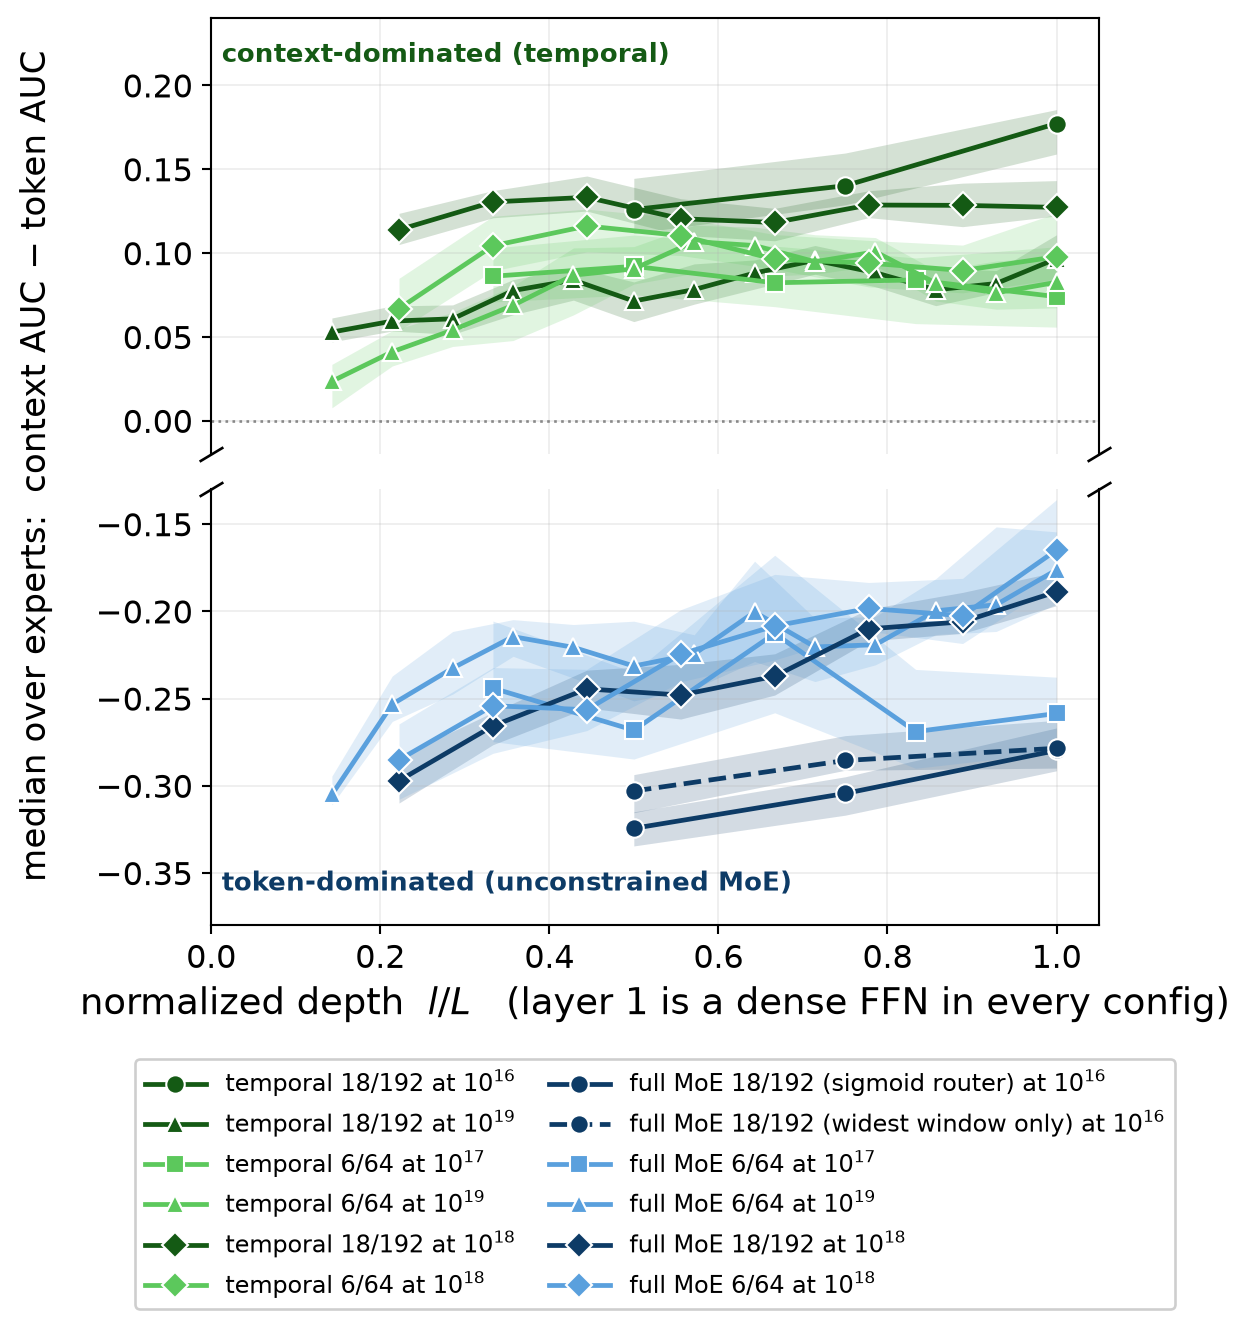
\includegraphics[width=0.62\linewidth]{figures/locus_by_layer_nocaption.png}
  \caption{Median context-minus-token AUC per MoE layer against normalized depth, one line
  per model, 95\% bootstrap bands. The broken axis reflects that the regime gap of about 0.3
  dwarfs the depth effect of about 0.05. One $10^{16}$ unconstrained model is the
  sigmoid-router control, and one was captured only at the widest context window (dashed).
  Unconstrained models climb with depth, temporal models start contextual and stay nearly
  flat.}
  \label{fig:locusdepth}
\end{figure}

\section{Serving measurement details}\label{app:serving}

\paragraph{Workstation protocol.} All RTX A6000 numbers use the llama.cpp CUDA fork of
Section~\ref{sec:serving} at Q4\_K\_M, four trials with the first discarded, decode over a
100-token generation after the prefill, and a perplexity gate that verifies the streaming
path bit-identical to the all-resident engine.

\paragraph{Micro-batch choice.} llama.cpp processes the prompt in micro-batches, and
Table~\ref{tab:ubatch} sweeps the size at 16k context. Figure~\ref{fig:servingctx} runs
both tiers at 2048, within 1\% of the all-resident time optimum and near the deploy VRAM
floor, so the setting flatters neither side. Larger micro-batches cost the deploy tier
much of its memory advantage because activation buffers grow with tokens in flight, and
smaller ones stall it.

\begin{table}[h]
  \centering\small
  \caption{Prefill micro-batch sweep at 16k context, fine-grained model. Time is prefill
  in ms (lower is better), memory is peak VRAM in MiB. Bold marks the operating point of
  Figure~\ref{fig:servingctx}.}
  \label{tab:ubatch}
  \vspace{4pt}
  \begin{tabular}{@{}rrrrr@{}}
    \toprule
    & \multicolumn{2}{c}{all-resident} & \multicolumn{2}{c}{deploy} \\
    \cmidrule(lr){2-3} \cmidrule(l){4-5}
    micro-batch & ms & MiB & ms & MiB \\
    \midrule
    1024  & 2975 & 8894  & 5527 & 3159 \\
    \textbf{2048}  & \textbf{2942} & \textbf{9512}  & \textbf{4499} & \textbf{3590} \\
    4096  & 2922 & 10746 & 4132 & 4986 \\
    16384 & 4723 & 18162 & 4247 & 13358 \\
    \bottomrule
  \end{tabular}
\end{table}

\paragraph{Where prefill time goes.} Three configurations at 16k context in one
micro-batch decompose the cost. The stock all-resident kernel takes 4715\,ms, the
expert-major kernel 4219\,ms with all experts resident and 4297\,ms streaming from the CPU
pool. Streaming is nearly free at every context, 1.00 to 1.05$\times$ the resident
control, so the deploy prefill cost is the kernel shape, 2.4$\times$ the stock kernel at
1k context and faster than it at 16k.

\paragraph{The vanilla-offload floor.} Figure~\ref{fig:floor} sweeps decode speed against
pinned cold expert fetches per layer per token, measured with real PCIe transfers on a
reconstruction of the serving models, and the rebuilt fine model reproduces the
all-resident ceiling at 200.8 tok/s. Free top-$k$ routing at active-only memory misses
$k(1-k/E)\approx16$ experts per layer at chance overlap and about 14 at the $\sim$20\%
consecutive overlap of released MoEs, which lands at 39 to 43 tok/s. Points at two or
fewer fetches are launch-bound and carry boost variance, and the bandwidth-bound floor is
stable.

\begin{figure}[h]
  \centering
  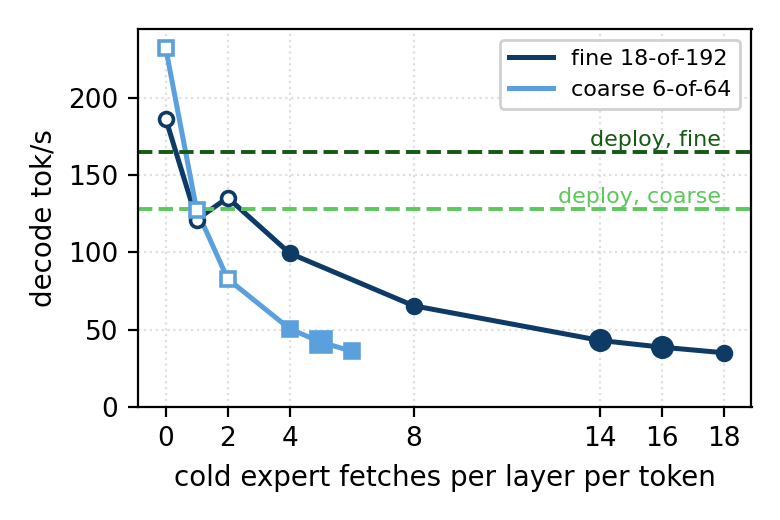
\includegraphics[width=0.6\linewidth]{figures/vanilla_floor_curve_nocaption.png}
  \caption{Decode speed against pinned cold expert fetches per layer per token. Hollow
  markers are launch-bound points, enlarged markers the rates behind
  Table~\ref{tab:serving}'s vanilla-offload row, dashed lines the temporal deploy rows at
  the same VRAM.}
  \label{fig:floor}
\end{figure}

\paragraph{Phone protocol.} The Pixel 10a runs a CPU slot pool with $R$ expert slots per
tensor in anonymous memory, evicting by releasing an expert's pages and fetching by direct
reads of the expert's exact bytes before its rows are computed, with four compute threads
and eight fetch workers on the 1+3+4 core topology. Two gates precede every recorded
number. Fetched bytes must match device-level disk counters, with agreement of 0.9 to
5\%, and perplexity must be bit-identical to the pool-disabled baseline through tens of
thousands of evict-and-refetch cycles. Decode measures 5.65 tok/s at $R=18$ (a
10.7$\times$ expert-memory cut), 10.49 at $R=36$ (5.3$\times$), 10.85 at $R=48$
(4$\times$), and 11.76 at $R=64$ (3$\times$), which is 32 to 71\% of an all-resident
ceiling of 16.6 to 17.5 tok/s inferred from byte accounting and stall-subtracted
cross-checks, since the all-resident model does not fit on the device. The random-weight
router changes 2.09 experts per layer per token, roughly twice the design point of a
trained temporal router, so the curve understates a trained model, most at the tightest
point.

\section{Instruct benchmark protocol}\label{app:instrproto}

\paragraph{Generation.} Every configuration samples with the model's own model-card recipe, seeded, in a
single pass at per-task budgets of 2048 tokens for non-thinking modes, 4096 for thinking,
and 8192 for thinking IFEval. An earlier truncate-and-retry ladder inflated scores by 2.6
points on average over 59 paired configurations and was retired for the single-pass protocol.
During generation only the end-of-sequence token stops the model, and task stop-strings
apply after the thinking block is stripped, since several fire inside chains of thought.

\paragraph{Scoring.} MMLU is dual-scored from the same generations. The stock strict
filter accepts only the form "The answer is (X)" and measures few-shot format imitation,
so the reported metric is relaxed answer extraction with final-answer-line priority.
HumanEval is parsed channel-aware per model family for models that think in-band, and
thinking text is never judged against task formats.

\paragraph{Instruments.} Full-grid configurations are single runs with binomial standard errors of 2 to
4 points. The Qwen3.5 adaptation evaluations are 200-item screening subsets compared only against same-batch
references, because constrained IFEval shows up to 8.6 points of batch-composition
sensitivity between item subsets. Free-routing MMLU at temperature 1.0 spreads up to 3.5
points across runs, so headline MMLU numbers use multi-run means.

\paragraph{WritingBench.} The official queries and critic model run locally through the
same constrained serving stack, three disjoint 50-query English subsets per configuration, scored 1
to 10 by the critic, with deltas paired within subset (paired standard deviations 0.05 to
0.15).

\paragraph{Displacement measures.} For Section~\ref{sec:instruct}'s predictor, router
displacement is the mean per-token total-variation distance between the router
distribution computed free and under the constraint on the same inputs, and functional
displacement is the relative output error of the routed-expert layer when the resident set
substitutes for the free choice,
$\lVert y_{\text{masked}}-y_{\text{free}}\rVert/\lVert y_{\text{free}}\rVert$, averaged
over layers. Figure~\ref{fig:displacement} plots both against mean benchmark damage at
$R=k$. Router displacement anti-orders damage (Spearman $-0.49$) while functional error
orders it ($+0.66$) and orders it exactly within each residency fraction. LFM contributes
its native thinking damage, having no off mode.

\begin{figure}[h]
  \centering
  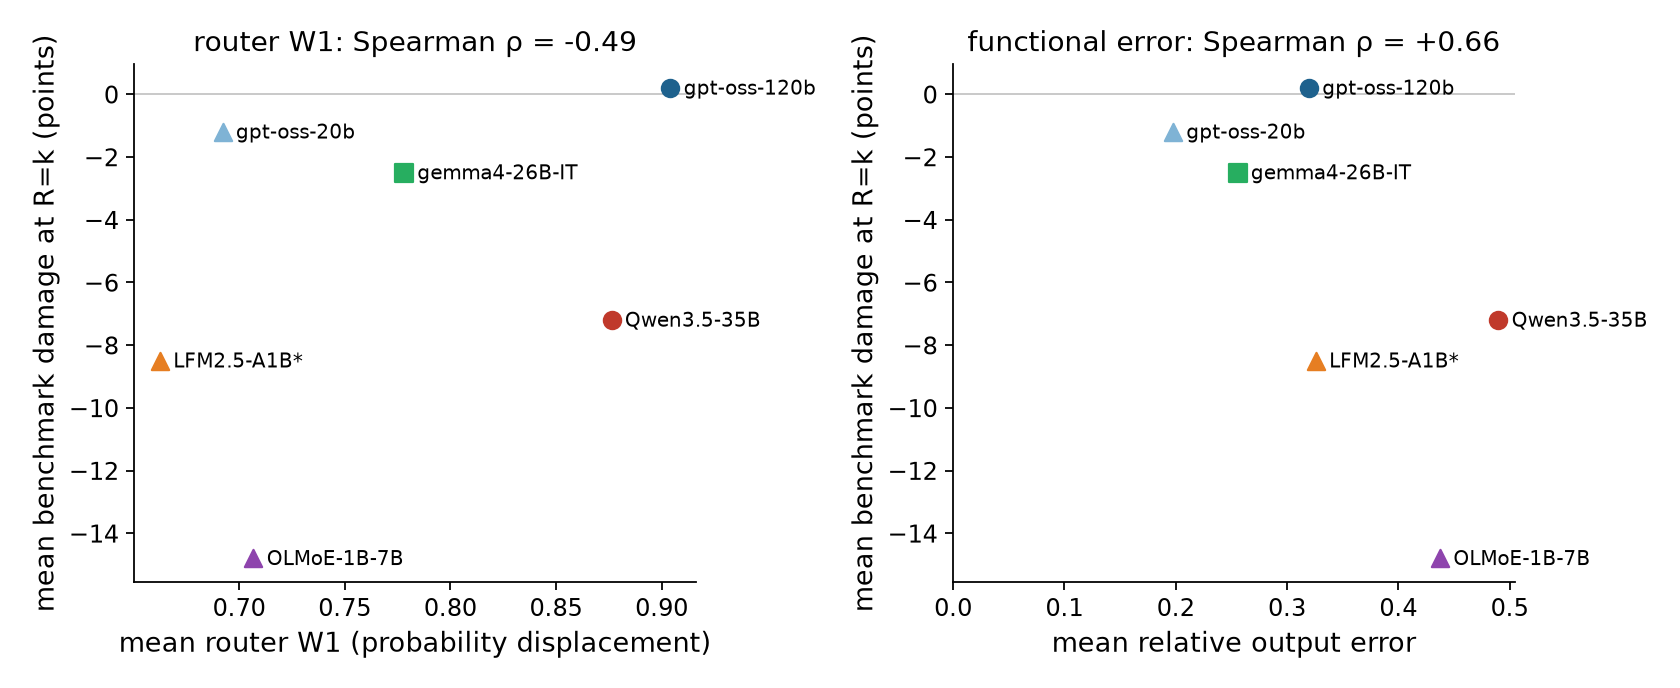
\includegraphics[width=0.9\linewidth]{figures/functional_displacement_nocaption.png}
  \caption{Mean benchmark damage at $R=k$ against router probability displacement (left)
  and functional displacement (right), one point per model, marker by residency fraction.
  The router-space measure anti-orders damage, the function-space measure orders it.}
  \label{fig:displacement}
\end{figure}

\section{Length analysis details}\label{app:length}

\paragraph{Data and definitions.} Length measurements pair the same items free and constrained
by document id with exact token counts, 200 items per configuration. GSM8K and IFEval carry
per-item capture, while MMLU and the family-specific HumanEval harnesses do not and are
absent rather than zero. A cap-hit is a generation within 8 tokens of its budget, and a
blow-up, the definition behind Section~\ref{sec:length}'s flip accounting, is a cap-hit or
a generation more than twice its paired counterpart. The decomposition of
Figure~\ref{fig:lendecomp} uses cap-hits only, so membership does not depend on the paired
length it decomposes.

\paragraph{Percentile detail.} Figure~\ref{fig:lenpct} gives the think-length ratio at
each percentile for all eighteen thinking configurations. The heterogeneity behind
Section~\ref{sec:length} is visible directly, with gemma4's growth concentrated at the tail
(P95 ratio 1.86 on GSM8K), gpt-oss-120b's at the median, and gpt-oss-20b shortening at
high effort. Ratios in configurations whose free-routing median thinking runs under about 100 tokens
are a few tokens of noise.

\begin{figure}[h]
  \centering
  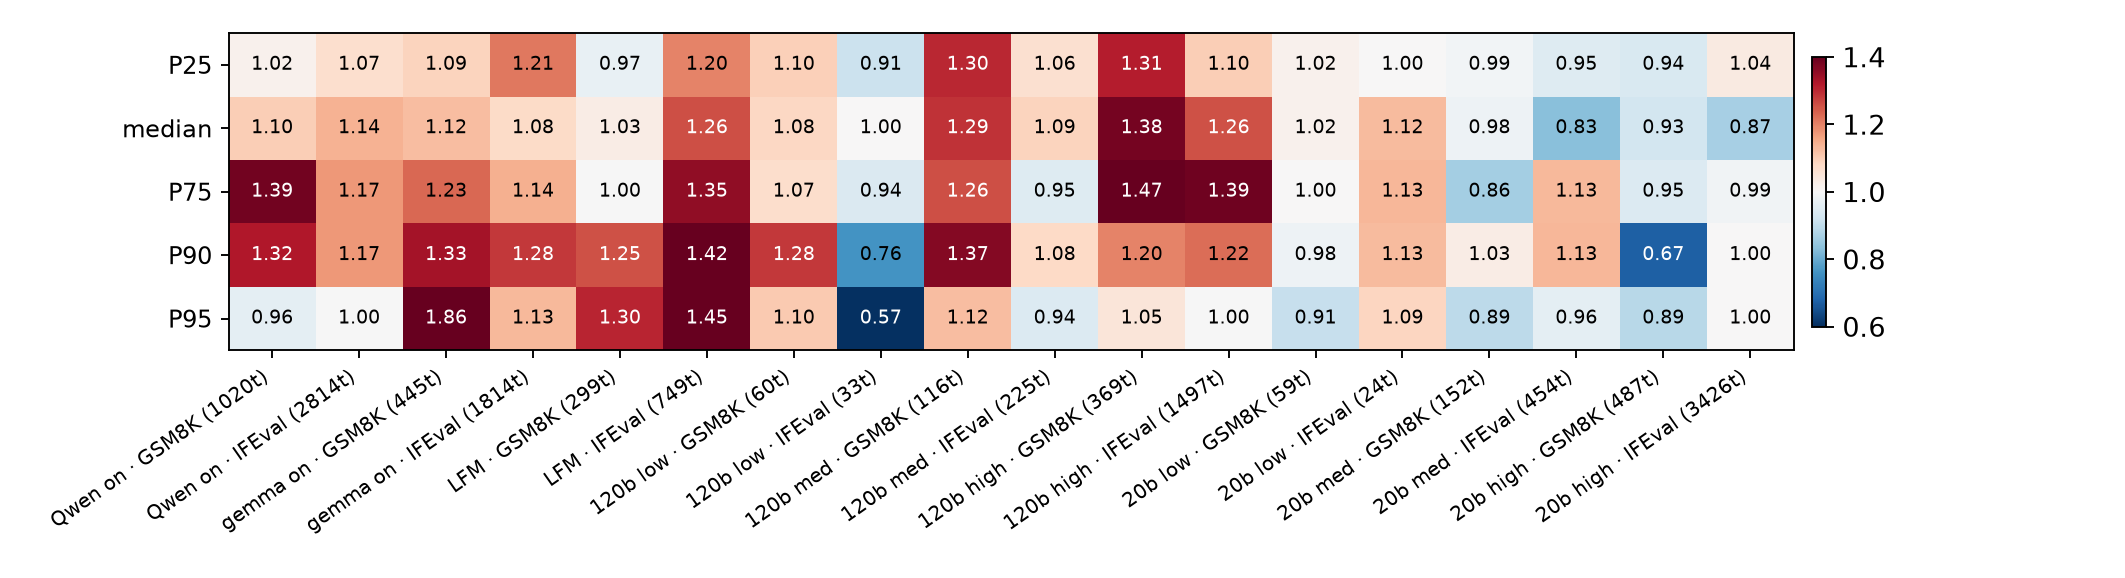
\includegraphics[width=\linewidth]{figures/length_percentiles_nocaption.png}
  \caption{Think-token ratio, tight cache over free, at five percentiles for every
  thinking configuration. Red is longer under the constraint, blue shorter, and each label carries
  the free-routing median think length in tokens.}
  \label{fig:lenpct}
\end{figure}

\paragraph{Flip accounting.} Across the ten thinking configurations the constraint flips 174 items
to wrong against 85 it rescues. On thinking IFEval, Qwen3.5 flips 35 items to wrong against 2 to
right, with 43\% of the wrong-flips blow-ups, and gemma4 flips 14 against 4 at 57\%, so the
net damage there is largely one-way traffic into blow-up. The gpt-oss models churn in both
directions at high effort, 14 wrong-flips against 13 rescues for 120b, netting almost
nothing. On GSM8K the wrong-flips are mostly normal length, with blow-up shares of 0 to
19\%, so that damage is quality loss rather than the budget wall. Blown-up items are wrong
more often than normal-length items in all 20 comparisons, the 10 thinking configurations crossed
with both settings, which is the basis for Section~\ref{sec:length}'s claim.

\paragraph{The length-damage null.} Figure~\ref{fig:lennull} plots damage at the tightest
setting against free-routing response length across tasks and models. No significant relationship
survives the corrected protocol (Spearman $-0.18$, $p=0.63$), and the earlier protocol's
significant correlation came from budget-truncated short-answer configurations and reconstructed
lengths.

\begin{figure}[h]
  \centering
  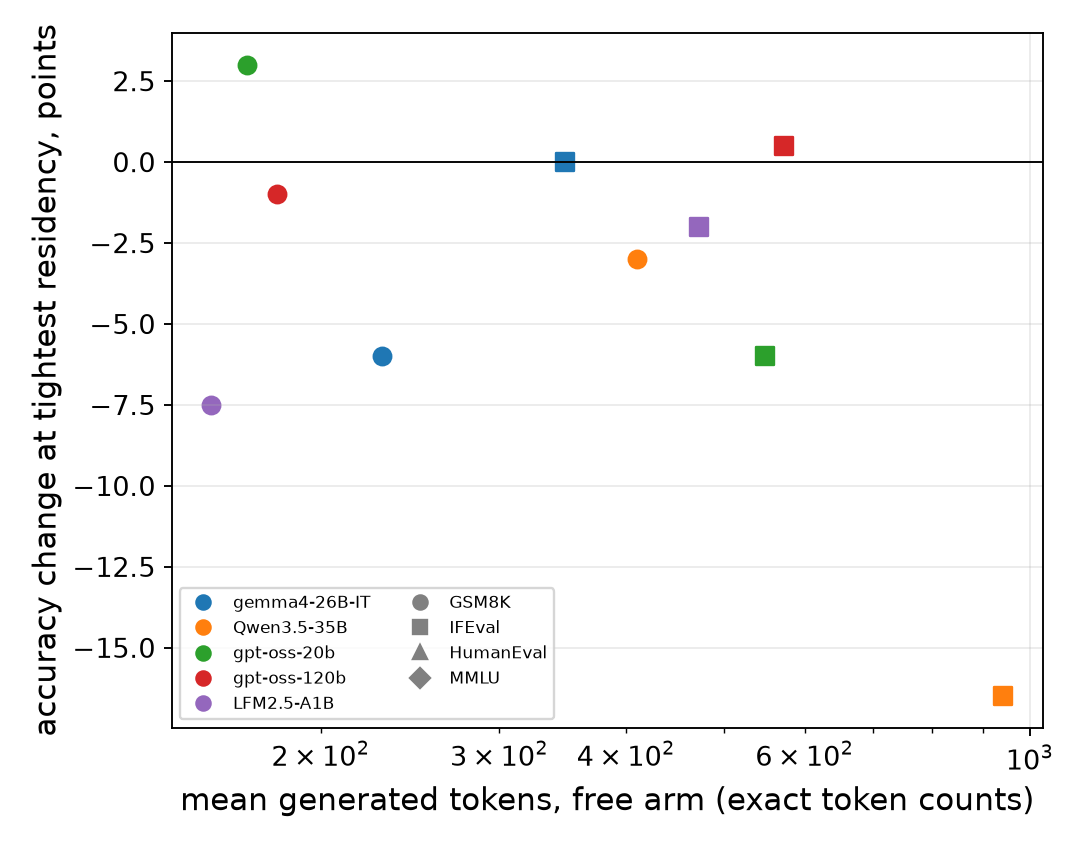
\includegraphics[width=0.55\linewidth]{figures/length_vs_damage_nocaption.png}
  \caption{Damage at the tightest residency setting against mean free-routing response length,
  color per model, marker per benchmark, exact token counts.}
  \label{fig:lennull}
\end{figure}

\end{document}
